% A compiler avec xelatex
\documentclass[11pt]{article}

\usepackage[utf8]{inputenc}
\usepackage[french]{babel}

% Pour inclure la page de garde
\usepackage{pdfpages}

%geometry of the page
\usepackage[vmargin=0.6in,hmargin=1in,showframe]{geometry}

\setlength{\parindent}{1cm}

%========================================= FONTS
\usepackage{fontspec}



\newcommand{\MEGA}{\fontsize{110}{-30}\fontspec{Mega:style=JDR-ORey}\selectfont}




% Police de caractères OD&D Saloon Girl Inline
%\newcommand{\ODDtitlefont}{\fontsize{38}{40}\fontspec{QuentinCaps}\selectfont}
\newcommand{\ODDtitlefont}{\fontsize{60}{40}\fontspec{Saloon Girl Inline}\selectfont}

% Police de caractères OD&D OPTIChisel-Normal:style=Regular
\newcommand{\ODDtitlebisfont}{\fontsize{52}{70}\fontspec{OPTIChisel-Normal:style=Regular}\selectfont}
\newcommand{\ODDsectionfont}{\fontsize{42}{50}\fontspec{OPTIChisel-Normal:style=Regular}\selectfont}

% Pour le PC 64 bits
\newcommand{\ODDtimes}{\fontspec{Times New Roman}\selectfont}
% Pour le PC 32 bits
%\newcommand{\ODDtimes}{\fontspec{Linux Libertine O}\selectfont}

%- \usepackage{xcolor}
\usepackage{titlesec}
\defaultfontfeatures{Ligatures=TeX}
% Set sans serif font to Calibri
%- \setsansfont{Calibri}

% Set main font
\setmainfont{Futura Std}

% Define light and dark Microsoft blue colours
%- \definecolor{MSBlue}{rgb}{.204,.353,.541}
%- \definecolor{MSLightBlue}{rgb}{.31,.506,.741}
% Define a new fontfamily for the subsubsection font
% Don't use \fontspec directly to change the font
%- \newfontfamily\subsubsectionfont[Color=MSLightBlue]{Times New Roman}
% Set formats for each heading level
%\titleformat*{\section}{\normalfont\fontsize{12}\ttfamily{QuentinCaps}}

%\titleformat{\section}{\fontspec{QuentinCaps}\selectfont}{\thesection}{1em}{}

\titleformat{\section}{\centering\ODDsectionfont}{\thesection}{1em}{}
\titleformat{\subsection}{\large\bfseries}{\thesubsection}{1em}{}


%- \titleformat*{\subsection}{\large\bfseries\sffamily\color{MSLightBlue}}
%- \titleformat*{\subsubsection}{\itshape\subsubsectionfont}

% pour le (R)
\usepackage{fontspec}

% Pour les images
\usepackage{graphicx}
\graphicspath{{./yed/}{./images/}{./maps/}}

% Array stretch pour avoir un peu plus de vertical spacing dans les tabular
\usepackage{tabularx}
\renewcommand{\arraystretch}{1.2}
\usepackage{multirow}

% Place les footnotes en bas et supprimer l'indentation dans la footnote
\usepackage[bottom]{footmisc}

%Macro pour réduire l'espace sous le titre
\newcommand{\myunderline}[1]{\underline{\smash{#1}}}

%++++++++++++++++++++++++++++++++++++++++++++++++++++++++++++++++++++++++++
%                               DOCUMENT
%++++++++++++++++++++++++++++++++++++++++++++++++++++++++++++++++++++++++++
\begin{document}

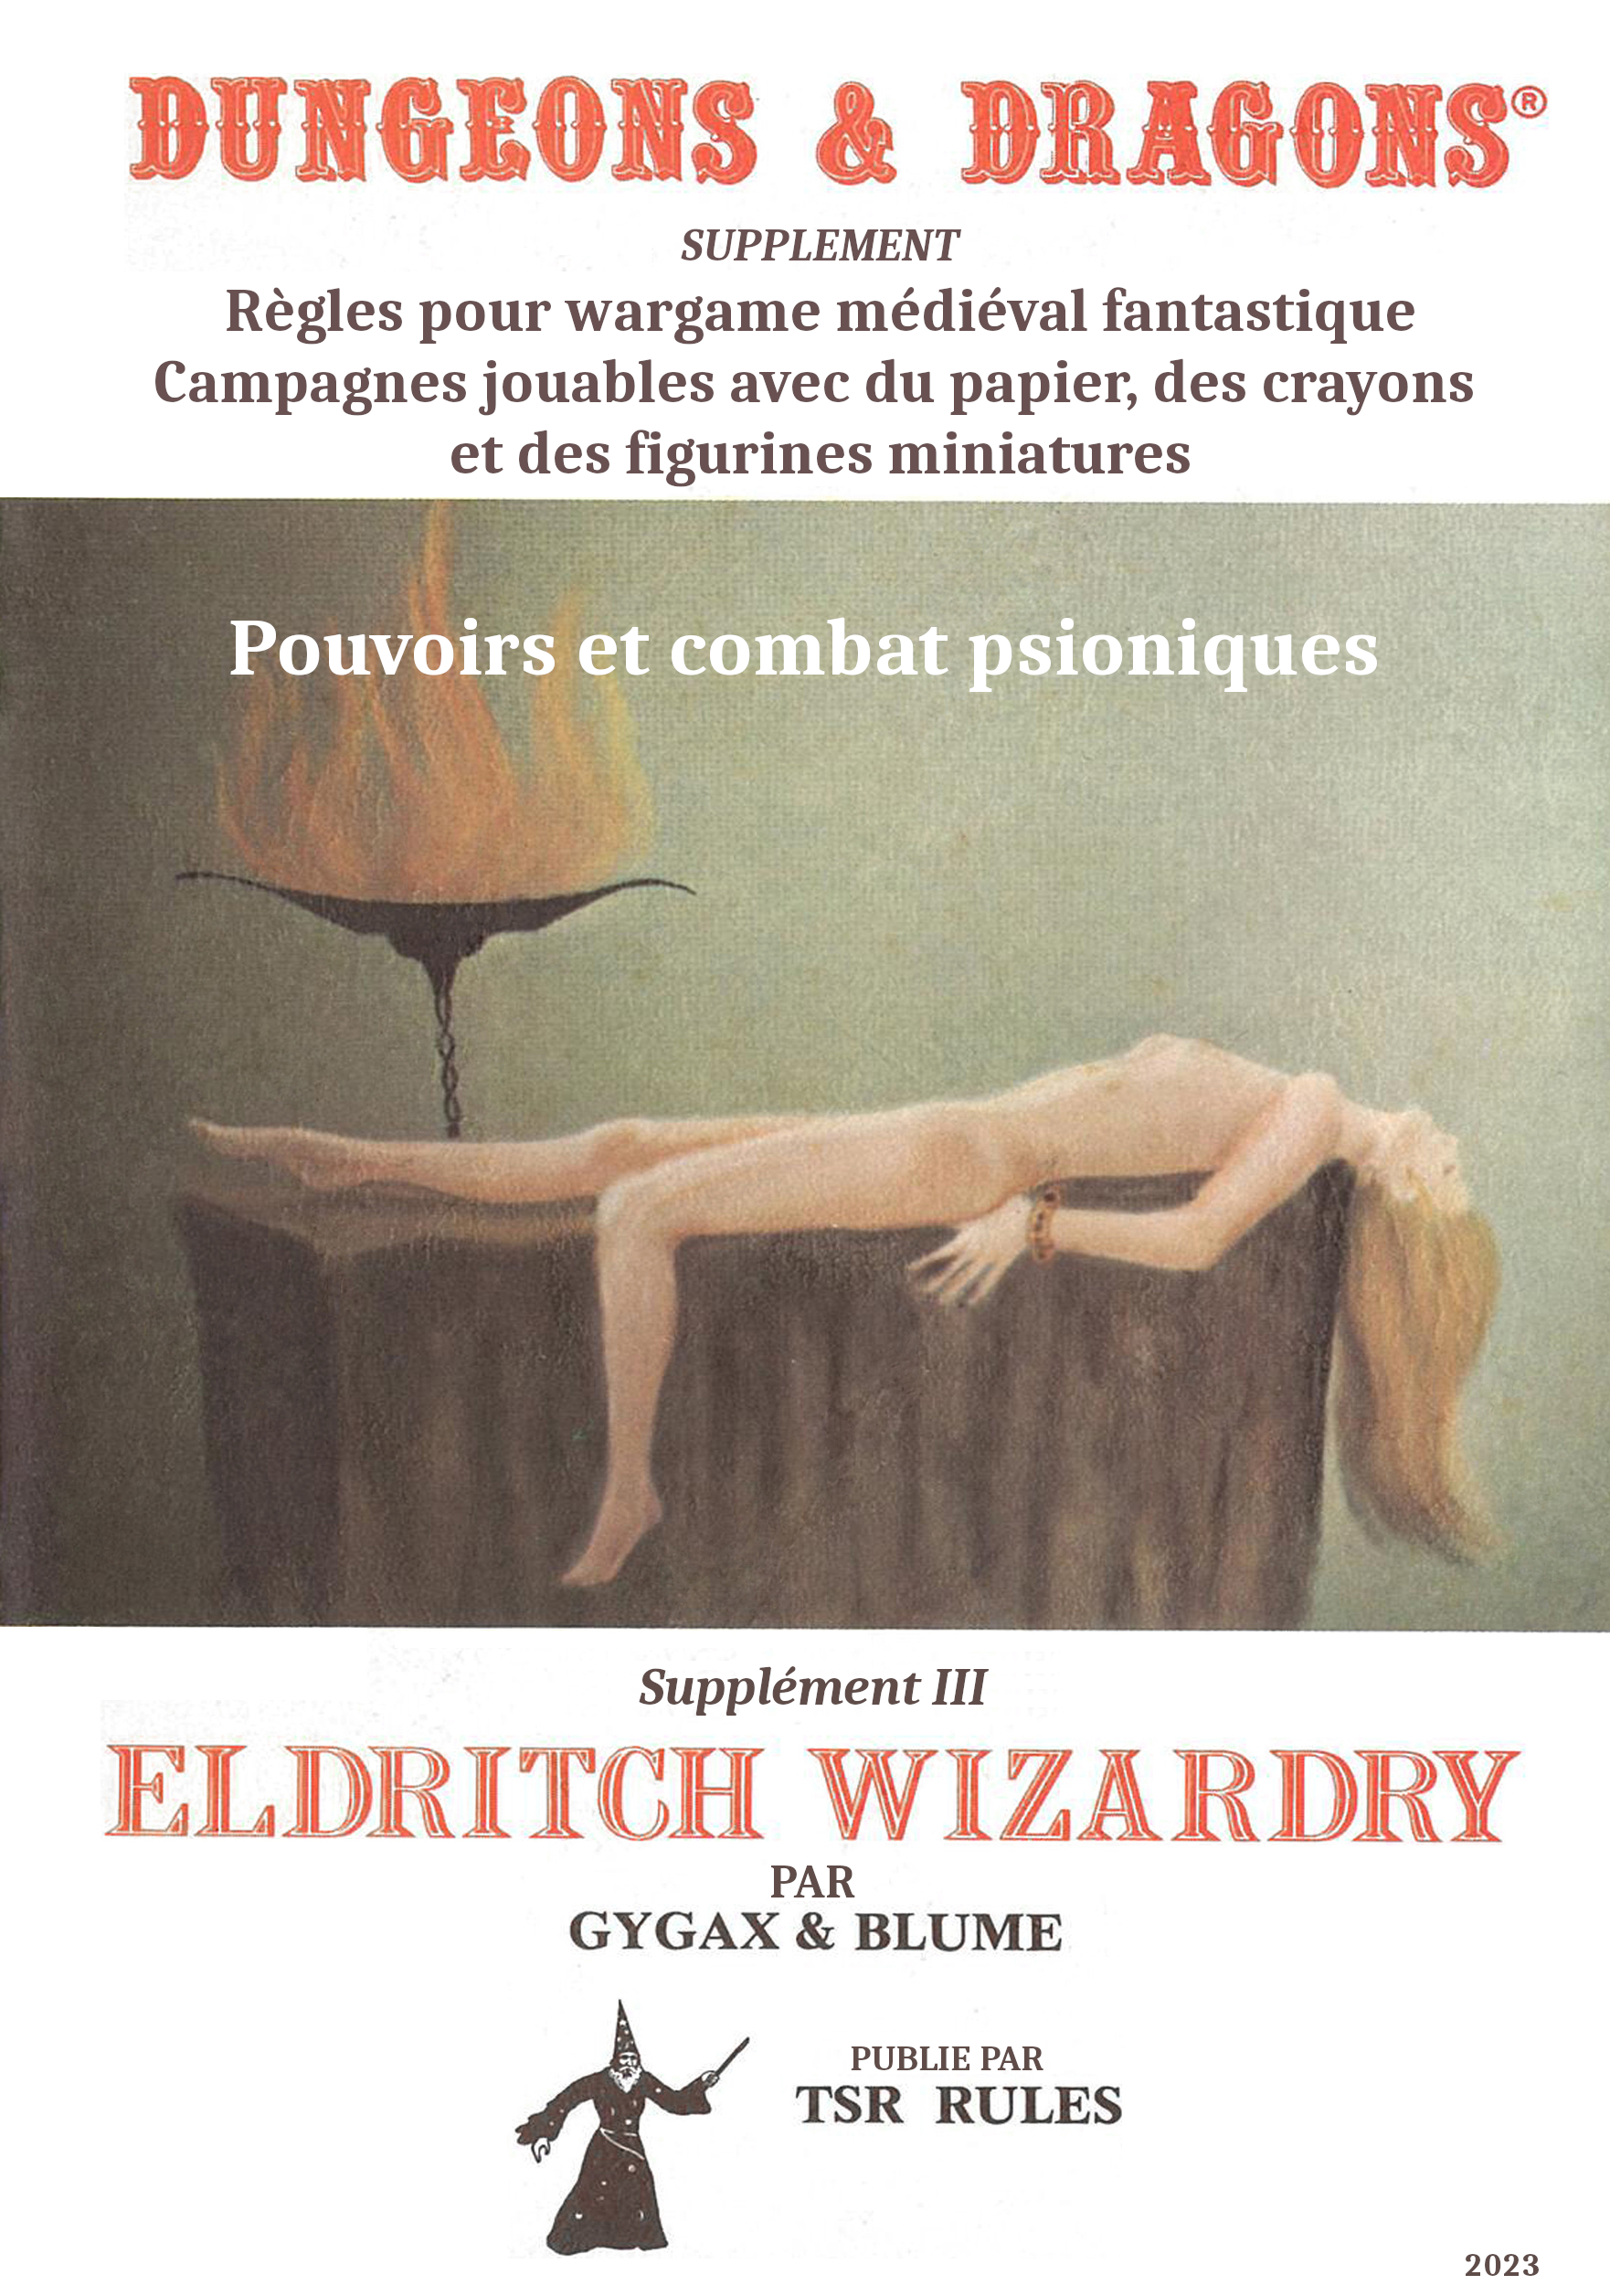
\includepdf[scale=0.9]{pagedegarde.pdf}
\newpage

{\color{white}a}

\newpage

\thispagestyle{empty}
\begin{center}
{\Huge \ODDtitlefont{DONJONS \& DRAGONS}}{\normalsize \textsuperscript{\sffamily\textregistered}}

\vspace{1.8cm}

{\Large \textbf{Supplément III}}

\vspace{1.3cm}

{\Huge \ODDtitlebisfont{ELDRITCH}}

\vspace{0.3cm}

{\Huge \ODDtitlebisfont{WIZARDRY}}

\vspace{2.0cm}

{\Large \textbf{MAGIE ANCIENNE ET PUISSANTE}}

\vspace{1cm}

{\large PAR

\vspace{0.1cm}

GARY GYGAX \& BRIAN BLUME

\vspace{3cm}

Remerciements spéciaux à l'aîné Steve Marsh, Dennis Sustare (le Super Druide),

Jim Ward \& Tim Kask pour leurs suggestions et contributions !

\vspace{0.8cm}

Illustrations de Dave Sutherland, Tracy Lesch \& Gary Kwapisz

Couverture par Deborah Larson}

\vspace{1.3cm}

\textbf{\ODDtimes{2023}}

\vspace{0.5cm}

\ODDtimes{\textbf{\textcopyright\ 1976 - TSR GAMES}

\textbf{9\textsuperscript{ème} impression, novembre 1979}

\textbf{Imprimé aux U.S.A}}
\end{center}

\vfill

{\small \noindent LES QUESTIONS SUR LES REGLES DOIVENT ETRE ACCOMPAGNEES D'UNE ENVELOPPE RETOUR TIMBREE ET ENVOYEES A TACTICAL STUDIES RULES, POB 756, LAKE GENEVA, WISCONSIN 53147}


\newpage
%====================================================
{\color{white}a}

\vfill

\noindent {\scriptsize \textit{Ce fascicule est une adaptation par Rouboudou (https://rouboudou.itch.io) de la partie pouvoirs psioniques du livret original. Cette adaptation est une œuvre de fan, gratuite et ne pouvant être vendue.}}

\newpage

\section*{Préface}

Le livre que vous tenez maintenant dans vos mains présente de nouvelles dimensions à un système de jeu déjà fascinant. Il s'agit du troisième supplément à DONJONS \& DRAGONS, produit comme conséquence à une demande toujours croissante de nouveau matériel.

Ce livre présente aussi une nouvelle mode dans l'art subtil d'être Maître de Donjon. Fidèle à sa conception d'origine, D\&D n'était limité dans son périmètre que par l'imagination et la dévotion des Maîtres de Donjons où qu'ils soient. Les suppléments ont répondu au besoin d'idées nouvelles et de mécanismes de simulation additionnels. Mais progressivement, D\&D a perdu un peu de sa saveur, et a commencé à devenir prévisible. Cela était dû à la prolifération d'ensembles de règles ; alors que c'était très bien pour nous en tant de compagnie, c'était compliqué pour le MD. Quand tous les joueurs avaient toutes les règles en face d'eux, il devenait presque qu'impossible de les séduire à affronter le danger ou les pièges.

Le nouveau concept innovant présenté dans ces pages devrait faire long feu en réintroduisant un peu de mystère, d'incertitude et de danger, qui refont de D\&D le défi sans équivalent qu'il a toujours été. La légende retrouve sa magie inestimable originale. On ne verra plus d'aventurier imprudent descendre dans un donjon , trouver quelque chose et savoir immédiatement ce que cela fait et comment cela fonctionne. De même, les joueurs ne pourront plus envoyer un de leurs infortunés serviteurs à une mort précoce en le forçant à expérimenter à sa place.

L'introduction du combat psionique est destiné à revivifier des parties devenues stagnantes. Il ouvre de nouvelles possibilités à la fois aux joueurs et au MD, tout en intégrant un des sujets favoris des auteurs de science-fiction et de fantastique : les pouvoirs inconnus de l'esprit.

Comme pour les deux précédents suppléments, le matériel contenu dans ce livret propose le même format que les trois livrets originaux de D\&D. Les corrections et les ajouts sont indiqués dans le texte de sorte qu'ils puissent être intégrés facilement dans les règles originales.

Comme vous pourrez le noter sur la page de titre, ce supplément est le fruit de plusieurs contributeurs. Telle est la nature de la chose que vous tenez entre vos mains. D\&D a été conçu pour être un jeu libre, lié aux règles de manière souple. Nous pensons que ELDRITCH WIZARDRY favorise les principes originaux de danger, d'excitation et d'incertitude. Que vous réussissiez toujours vos jets de sauvegarde.

\vspace{1cm}

\noindent Timothy J. Kask

\noindent TSR Publications Editor

\noindent Lake Geneva, Wisconsin

\noindent 23 avril 1976

\newpage

\section*{Introduction}

Le terme anglais \texttt{psionic} a été utilisé la première fois en 1951 dans une nouvelle de science-fiction écrite par Jack Williamson, \texttt{The Greatest Invention}, publié dans le magazine \texttt{Astounding Science Fiction}. Il est la compression de deux deux termes, \texttt{psi} dans le sens de phénomène psychique et \texttt{electronics}. \texttt{Psionics} devient un terme décrivant la discipline qui étudie les phénomènes psychiques avec les moyens de l'ingénierie moderne de l'époque, soit l'électronique. Malgré la promotion de personnes comme John W. Campbell, le terme restera utilisé uniquement dans le monde de la science-fiction, avant d'être intégré dans le monde des jeux de rôles.

La version originale de Donjons \& Dragons, dite OD\&D, est publiée en 1974 sous la forme de trois livrets à la couverture marron. On trouve dans le second livret, \texttt{Monsters and Treasures}, les premières références à des pouvoirs psychiques, dans la section traitant des épées magiques. A l'époque, le terme \texttt{psionic} n'est pas utilisé.

En 1976, dans le deuxième supplément \texttt{Eldritch Wizardry} cosigné par Gary Gygax et Brian Blume, les pouvoirs psychiques arrivent dans le monde des personnages-joueurs et des personnages-non-joueurs. Les règles sont présentées de manière assez chaotique, ce qui générera vite la réputation d'un système injouable dans le monde des joueurs. Derrière la juste critique sur la présentation, beaucoup de joueurs semblent avoir rejeté le supplément en raison du fait même de proposer, en extension à un jeu médiéval-fantastique, une gestion des pouvoirs mentaux, habituellement présents dans les univers de science-fiction.

Nous proposons ici une double présentation des règles psioniques du supplément \texttt{Eldritch Wizardry} : le premier chapitre propose les règles originales traduites le plus fidèlement possible ; le chapitre suivant propose une réorganisation de ces règles visant à les présenter de manière plus claire et plus logique. La consultation de certains sites américains a été nécessaire pour s'assurer de la bonne compréhension de certaines règles ambiguës qui, encore aujourd'hui, provoquent des commentaires et des incompréhensions.

Une fois éclairci, le système se montre très intéressant, non seulement parce qu'il est très "gygaxien" (on le voit notamment au travers de l'utilisation de règles gigognes), mais aussi parce qu'il est le premier système complet de psioniques proposant une façon nouvelle de voir les pouvoirs, très différente de la magie de OD\&D, façon qui inspirera beaucoup d'autres systèmes de pouvoirs dont l'utilisation est basée sur la consommation de points.

Dans la partie \texttt{Monstres et Trésors}, nous proposons une traduction des règles concernant les épées magiques (psioniques), règles extraites du second livret, \texttt{Monsters and Treasures}, de OD\&D.

\vspace{1cm}

\noindent Rouboudou

\noindent https://orey.github.io/blog

\noindent Juillet 2023

\newpage

\section*{Index}

\newpage

%==========================================================================SECTION
\section*{Hommes \& Magie}

\subsection*{{\normalsize PERSONNAGES :}}

{\parindent0pt

Il existe une catégorie spéciale de personnages qui traverse les quatre classes majeures de personnages-joueurs. Ceux qui possèdent des \textbf{capacités psioniques} peuvent être trouvés parmi les combattants, les magiciens, les clercs et même les voleurs.

\bigskip

Plus de détails concernant les capacités psioniques et comment déterminer sur ce potentiel existe seront trouvés dans la section \textbf{DETERMINATION DES CAPACITES}.

\bigskip

Il est important de garder à l'esprit ce qu'est un \og monstre \fg{}. Pour le jeu D\&D, un monstre est toute entité contrôlée par le MD. Les personnages-joueurs et les personnages-non-joueurs contrôlés par les joueurs ne sont pas des monstres : tout le reste, par contre, l'est. Un monstre à D\&D peut être n'importe quoi depuis un démon de Type VI jusqu'à un clerc gentiment Loyal Bon.

\bigskip

Tous les joueurs avec des aptitude psioniques doivent être humains.

\bigskip

Les \textbf{combattants} sont essentiellement sensibles aux pouvoirs communément connus sous le nom de Yoga. Il y a 20 \og dévotions \fg{} possibles qu'ils peuvent accomplir (les 18 Siddhis et les 2 Sciences) s'ils suivent le développement de leurs talents mentaux. Cependant, pour \textbf{chaque} aptitude qu'ils gagnent, ils doivent perdre un de leurs suivants et un point de Force est perdu de manière permanente pour chaque ensemble de \textbf{quatre} aptitudes. (De plus, ils deviennent sensibles à certains types de monstres et aux attaques de monstres que les personnages sans capacités psychiques ne subissent pas, comme cela sera détaillé plus tard).

\bigskip

Les \textbf{magiciens} qui ont des aptitudes psioniques verront que cela élimine la nécessité d'apprendre certains sorts qui leur donnent fondamentalement les mêmes pouvoirs pour une durée limitée. C'est une chance, car pour chaque aptitude psionique gagnée, le magicien perdra la capacité de se souvenir d'un sort. Cela implique qu'avec le gain de la première aptitude, le magicien sera capable d'utiliser un sort de premier niveau de moins ; quand la deuxième aptitude sera gagnée, il perdra deux niveaux de sorts \textbf{de plus} (soit deux sorts de premier niveau ou un sort de deuxième niveau), et ainsi de suite. Jamais le magicien ne doit se souvenir de plus de sorts de haut niveau que de sorts de bas niveau, et s'il est capable d'utiliser des sorts du sixième niveau, il doit être capable de se souvenir d'au moins un sort de tous les autres cinq niveaux. Les attaques des créatures psioniques seront aussi subies par les magiciens qui développent ce talent.

\bigskip

Les \textbf{clercs} ayant des aptitudes psioniques gagnent aussi l'avantage de pouvoir employer plusieurs pouvoirs \og magiques \fg{}, mais pour chaque aptitude psionique gagnée, le clerc perdra deux de ses autres avantages : primo, il perdra un sort, de la même façon que le magicien ; secundo, le clerc perd la capacité de retourner les morts-vivants à mesure qu'il gagne des pouvoirs  psioniques, de sorte que pour chaque aptitude psionique gagnée, le clerc se place un niveau plus bas dans la capacité de retourner les morts-vivants. Ainsi, un clerc de niveau 10 avec quatre aptitudes psioniques aura perdu 10 niveaux de sorts\footnote{Les pertes de niveaux de sorts sont cumulatives. Pour le gain de 4 aptitudes psioniques : 1 (niveau 1) + 2 (niveau 2) + 3 (niveau 3) + 4 (niveau 4) = 10 niveaux de sorts seront perdus (NdT).} et retournera les morts-vivants comme un clerc de niveau 6. Gagner des aptitudes psioniques rend aussi la personne disposant de ces capacités sensible aux attaques des créatures psioniques.

\bigskip

\textbf{Les moines \& les druides n'ont pas de potentiel psychique : il leur est donc interdit de devenir des personnes aux pouvoirs psychiques.}

\bigskip

Les \textbf{voleurs} qui ont un potentiel psychique avéré sont sujets aux mêmes avantages que ceux gagnés par les combattants. Néanmoins, en plus des pénalités notées pour les combattants, les voleurs perdent aussi 1 point de dextérité toutes les quatre aptitudes gagnées.

\subsection*{{\normalsize DETERMINATION DES APTITUDES :}}

\medskip

Après que les six caractéristiques normales ont été tirées, et que le joueur a choisi un type de personnage, les personnages-joueurs qui disposent d'un score non modifié de 15 ou plus en Intelligence, Sagesse ou Charisme peuvent choisir, en plus, de tester leur capacité psionique, s'ils ont fait le choix d'être humain. La capacité psionique est déterminée en faisant un jet de pourcentage. Un score de 91 ou plus indique que le personnage a cette capacité.

\bigskip

\textbf{Bonus et pénalité à l'avancement dus aux aptitudes :}

\bigskip

Les personnages-joueurs avancent en niveaux comme indiqué par leur classe et leur caractéristique principale. La capacité psionique, néanmoins, est affecté par le potentiel psychique. Un second jet de dés doit être fait pour déterminer ce niveau, ainsi que les bonus et pénalités afférents :

\bigskip

{\parindent3cm POTENTIEL PSYCHIQUE

\bigskip

\begin{tabular}{p{3cm}l}
\textbf{Score} & \textbf{Bonus ou pénalité} \\
\textbf{des dés} & \textbf{Chance de gagner une aptitude} \\
01--10 & --6\%/niveau cumulatif \\
11--25 & --5\%/niveau cumulatif \\
26--50 & --4\%/niveau cumulatif \\
51--75 & Aucun \\
76--90 & +1\%/niveau cumulatif \\
91--99 & +2\%/niveau cumulatif \\
\hspace{0.4cm}00 & +3\%/niveau cumulatif \\
\end{tabular}}

\bigskip

Si un personnage a une pénalité de --4\%, sa chance de base de gagner une aptitude sera de 6\% au lieu de 10\%\footnote{La chance de base est de 10\% par niveau, de manière cumulative (NdT).}. De même, si son bonus est de 3\%, sa chance de base par niveau sera de 13\%, si bien qu'au niveau 3, la chance de gagner une aptitude psionique sera de 39\%.

\bigskip

\textbf{Bonus} : si une aptitude psionique est gagnée, la chance de gagner immédiatement une seconde aptitude est égale au potentiel psychique du personnage.

\begin{center}
\includegraphics[scale=0.17]{./images/demon-typeVI.jpg}
\end{center}

\subsection*{\normalsize NIVEAUX ET POINTS D'EXPERIENCE POUR LES ATTEINDRE}

Les personnages-joueurs possédant des aptitudes psioniques progressent de la façon standard dans le type de personnage qu'ils ont choisi au départ. Néanmoins, à partir du niveau~1, ils ont la possibilité d'acquérir une aptitude de type psionique. Les aptitudes psioniques sont listées dans la section \textbf{SORTS}. La probabilité de gagner une aptitude est de 10\% par niveau d'expérience, de sorte qu'un personnage de niveau 1 dispose d'une chance de 10\% d'avoir une aptitude psionique, un personnage de niveau 2 aura 20\% de chances, et ainsi de suite jusqu'au personnage de niveau 10ayant 100\% de chances.

\bigskip

La sélection de l'aptitude de type psionique est faite aléatoirement, mais si le sort indique une aptitude déjà possédée, il est nécessaire de rejouer  jusqu'à ce qu'une aptitude non possédée par le personnage soit tirée. Quand le personnage dispose de 100\% de chances de gagner une aptitude (10\textsuperscript{ème} niveau), le personnage peut choisir n'importe quelle aptitude quand il gagne un niveau d'expérience.

\subsection*{\normalsize COMBAT PSIONIQUE}

Il y a basiquement deux formes d'attaque psionique: 1) la forme dans laquelle il n'y a pas d'attaque en retour et 2) la forme qui est un échange d'attaques et de défenses où deux créatures avec des aptitudes psioniques sont impliquées. Certains dispositifs magiques ou aptitudes psioniques limitées modifieront le cas 1) ci-dessus. Il est aussi possible que certaines créatures dotées d'aptitude psioniques aient une forme d'attaque qui affectera uniquement les autres formes de vie dotées de capacités psioniques. Quand le combat psionique se produit, aucune autre action ne peut être effectuée.

\medskip

Les attaques psioniques sur les créatures non-psioniques ne peuvent être faites que si l'attaquant a une force d'attaque psionique de plus de 120. La force d'attaque psionique est déterminée en additionnant le \textbf{potentiel psychique} au nombre d'aptitudes psioniques multiplié par deux et le nombres de modes d'\textbf{attaques psioniques} et de \textbf{défenses psioniques} multiplié par cinq. Par exemple, un personnage avec un potentiel psychique de 37, 6 aptitudes psioniques et 5 modes d'attaques et de défenses aurait une force d'attaque psionique de 73 (37 + 12 (6x2) + 25 (5x5)). Les dépenses précédentes en points de force psionique sont considérées avec un ratio de 50\%, ce qui fait qu'un usage de 12 points réduit la force d'attaque de 6 points. Les forces d'attaque psionique des monstres sont exposées dans les paragraphes traitant des monstres dotés de pouvoirs psioniques.

\medskip

Après avoir fait la première attaque, ou dans le cas où les opposants annoncent simultanément qu'ils attaquent de manière psionique (ou dans le cas où le monstre le fait automatiquement et le personnage annonce qu'il le fait), la séquence d'attaque est déterminée comme suit : chaque opposant fait un jet de pourcentage et ajoute le résultat à sa force d'attaque psionique. Le plus haut score attaque en premier.

\bigskip

{\parindent0.5cm
\begin{tabular}{llcll}
\multicolumn{2}{l}{\textbf{Modes d'attaque, toutes classes}} && \multicolumn{2}{l}{\textbf{Modes de défense, toutes classes}} \\
A. & Onde de choc psionique (20)  && F. & Esprit vide (1) \\
B. & Poussée de l'esprit (10) 	  && G. & Bouclier de pensées (2) \\
C. & Coup de fouet sur l'ego (15) && H. & Barrières mentales (4) \\
D. & Imposition d'identité (10)   && I. & Forteresse intellectuelle (7) \\
E. & Écrasement psychique (25*)   && J. & Tour de volonté de fer (10) \\
&&&& \\
\multicolumn{5}{p{15cm}}{(Le coût d'utilisation en points de force psionique est montré entre parenthèses)} \\
\multicolumn{5}{p{15cm}}{*Si le joueur possède moins de points, altérer la probabilité de succès en \% en conséquence} \\
\end{tabular}}

Tout personnage doué de pouvoirs psychiques gagne immédiatement son premier mode d'attaque (onde de choc psionique) dès qu'il gagne sa première aptitude. Les aptitudes devraient être sélectionnées aléatoirement, mais un personnage ne devrait \textbf{jamais} avoir plus d'aptitudes supérieures que d'aptitudes basiques. Dans la sélection aléatoire, il est suggéré de mettre un poids supérieur aux probabilités de gain d'aptitudes liées à des aptitudes déjà possédées, par exemple empathie augmenterait les chances de gagner ESP, télépathie animale et projection télépathique. Les modes d'attaques additionnels sont gagnés à hauteur de un à chaque quatre aptitudes (cinq pour les combattants). La force psionique totale est deux fois la force d'attaque psionique (ou la force psionique d'attaque et de défense additionnées).Pour les détails sur la restauration des points de force psionique, se référer à la section FORCE PSIONIQUE. %TODO vérifier que cette section existe

\subsection*{\normalsize MODES DE D'ATTAQUE ET DE DEFENSE PSIONIQUES}

\begin{tabular}{p{5cm} >{\centering\arraybackslash}p{2.5cm}>{\centering\arraybackslash}p{2.5cm}>{\centering\arraybackslash}p{2.5cm}}
&\multicolumn{3}{c}{\textbf{Portée}} \\
\textbf{Mode d'attaque} & \textbf{Courte} & \textbf{Moyenne} & \textbf{Longue} \\
Écrasement psychique & 2m & -- & -- \\
Onde de choc psionique & 1m & 2.5m & 4m \\
Poussée de l'esprit & 3m & 6m & 9m \\
Coup de fouet sur l'ego & 2m & 4m & 6m \\
Imposition d'identité & 4m & 8m & 12m \\
\end{tabular}

\medskip

La portée courte augmente de 0.3m (et les autres portées augmentent de la même façon proportionnellement) avec chaque niveau de maîtrise d'une capacité d'attaque.

\medskip

Les attaques à portée moyenne font seulement 80\% des dommages précisés. Les attaques à longue portée font seulement 50\% des dommages précisés.

\bigskip

\begin{tabular}{p{7.5cm}p{6cm}}
\textbf{Mode de défense} & \textbf{Protection maximale pour} \\
Esprit vide & Individu seul \\
Bouclier de pensées & Individu seul \\
Barrière mentale & Individu seul \\
Forteresse intellectuelle & Cercle de 3m autour de l'individu \\
Tour de volonté de fer & Cercle de 1m autour de l'individu \\
\end{tabular}

\bigskip

Les attaques sur un individu surpris sont gérées dans la MATRICE DES ATTAQUES PSIONIQUES SPECIALES.

\medskip

\begin{tabular}{c>{\centering\arraybackslash}p{1.6cm}>{\centering\arraybackslash}p{1.6cm}>{\centering\arraybackslash}p{1.6cm}>{\centering\arraybackslash}p{1.6cm}>{\centering\arraybackslash}p{1.6cm}>{\centering\arraybackslash}p{1.6cm}>{\centering\arraybackslash}p{1.6cm}}
\textbf{Force} &&&&&& \\
\textbf{d'attaque} & \multicolumn{7}{c}{\textbf{Potentiel psionique du défenseur}} \\
\textbf{psionique} & \textbf{01--10} & \textbf{11--25} & \textbf{26--50} & \textbf{51--75} & \textbf{76--90} & \textbf{91--99} & \textbf{00} \\
01--20      & S & S & 40 & 30 & 20 & 10 & 5 \\
21--40      & S & S & S  & 40 & 30 & 20 & 10 \\
41--60      & W & S & S  & S  & 40 & 30 & 20 \\
61--80      & W & S & S  & S  & S  & 40 & 30 \\
81--90      & C & W & S  & S  & S  & S  & 40 \\
91--00      & C & C & W  & S  & S  & S  & S \\
101--110    & D & C & C  & W  & S  & S  & S \\
111--120    & D & D & C  & C  & W  & W  & S \\
121 et plus & D & D & D  & C  & C  & C  & W \\
\end{tabular}

\bigskip

\begin{tabular}{lp{14.5cm}}
S = & Etourdi pour 5--20 tours, pas d'attaque psionique \\
W = & Blessure psychique, récupération en 1--6 mois, pas d'attaque psionique \\
C = & Handicapé psionique de manière permanente, perd toutes ses aptitudes \\
D = & Mort \\
5--40 = & Nombre de points d'attaque psionique perdu -- récupérés en 1--6 jours \\
Note : & L'attaque Coup de fouet sur l'ego qui donne un résultat "D" veut dire stupidité et le résultat "C" doit être considéré comme "W". L'attaque Imposition psychique avec un résultat de "W", "C", ou "D" signifie que le défenseur est sous le contrôle de l'attaquant jusqu'à ce qu'il soit libéré. \\
\end{tabular}

\subsection*{\normalsize MATRICE A : ATTAQUE PSIONIQUE SUR NON-PSIONIQUE}

\begin{tabular}{c>{\centering\arraybackslash}p{2.6cm}>{\centering\arraybackslash}p{2.6cm}>{\centering\arraybackslash}p{2.6cm}l}
\textbf{Intelligence} & \multicolumn{3}{c}{\textbf{Jet de sauvegarde par portée d'attaque}} & \textbf{EFFET SI SAUVE-} \\
\textbf{du défenseur} & \textbf{Courte} & \textbf{Moyenne} & \textbf{Longue} & \textbf{GARDE ECHOUEE} \\
3--4    & 19 & 18 & 17 & Mort \\
5--7    & 17 & 16 & 15 & Coma 1--4 jours \\
8--10   & 15 & 14 & 13 & Sommeil 20--120 min. \\
11-12   & 13 & 12 & 11 & Etourdi 1--4 tours \\
13-14   & 11 & 10 &  9 & Confus 1--6 tours \\
15-16   &  9 &  8 &  7 & Furieux 1--8 tours \\
17      &  7 &  6 &  5 & Esprit affaibli \\
18      &  5 &  4 &  3 & Folie permanente \\
19      &  3 &  2 &  1 & Folie 1--4 semaines \\
20 \& + &  1 &  0 & -1 & Folie 2--12 jours \\
\end{tabular}

\bigskip

AJUSTEMENTS AU JET DE SAUVEGARDE :

\medskip

\begin{tabular}{p{4cm}c p{2.8cm} p{6.5cm} l}
\multicolumn{2}{c}{\textbf{Ajouts au dé}} && \multicolumn{2}{c}{\textbf{Soustractions au dé}} \\
Magicien & +1 && Médaillon ESP & -5 \\
Clerc    & +2 && Sort relié aux pouvoirs psioniques* & -4 \\
Elfe     & +2 && Etourdi & -3 \\
Nain     & +4 && Confus & -2 \\
Halfling & +4 && Enragé & -1 \\
Heaume télépathique & +4 && Esprit affaibli & ** \\
&&& Fou & *** \\
\end{tabular}

\begin{tabular}{rp{15.3cm}}
* & Voir la liste des aptitudes psionique plus loin pour comparaison \\
** & Traiter un esprit affaibli comme une personne à l'intelligence de 3--4 \\
*** & Les individus fous ne peuvent être attaqués psioniquement que par l'"Imposition" (voir la section APTITUDES PSIONIQUES).
\end{tabular}

\medskip

Un heaume de télépathie porté par le défenseur \textbf{étourdira} l'attaquant pour trois tours si le défenseur réussit son jet de sauvegarde.

\subsection*{\normalsize MATRICE B : COMBAT PSIONIQUE COMPLET, AVEC DOMMAGES}

\begin{tabular}{clccccc}
\small\textbf{Force} & & \multicolumn{5}{c}{\small\textbf{Mode défensif}} \\
\small\textbf{psionique} & \small\textbf{Mode} & \small\textbf{Esprit} & \small\textbf{Bouclier} & \small\textbf{Barrière} & \small\textbf{Forteresse} & \small\textbf{Tour de vo-} \\
\small\textbf{totale} & \small\textbf{offensif} & \small\textbf{vide} & \small\textbf{de pensées} & \small\textbf{mentale} & \small\textbf{intellectuelle} & \small\textbf{lonté de fer} \\
21 & Onde       &    3 & 7    & 4 & 2 & 0 \\
   & Poussée    &   12 & 5    & 1 & 0 & 3 \\
à  & Fouet      &    8 & 4    & 0 & 0 & 0 \\
   & Imposition &    2 & 5    & 8 & 1 & 2 \\
40 & Écrasement & 02\% & 01\% & - & - & - \\

41 & Onde       &    4 & 9    & 5    & 3 & 0 \\
   & Poussée    &   14 & 7    & 02   & 1 & 4 \\
à  & Fouet      &   10 & 6    & 0    & 0 & 0 \\
   & Imposition &    3 & 7    & 10   & 3 & 4 \\
60 & Écrasement & 04\% & 02\% & 01\% & - & - \\

61 & Onde       &    6 & 11   & 7    & 4    & 0 \\
   & Poussée    &   16 & 9    & 4    & 2    & 5 \\
à  & Fouet      &   13 & 9    & 1    & 0    & 1 \\
   & Imposition &    4 & 9    & 13   & 5    & 7 \\
80 & Écrasement & 08\% & 04\% & 02\% & 01\% & - \\

81 & Onde       &    9 & 14   & 9    & 5    & 0  \\
   & Poussée    &   18 & 11   & 6    & 3    & 6  \\
à  & Fouet      &   17 & 13   & 2    & 0    & 2  \\
   & Imposition &    6 & 11   & 16   & 8    & 10 \\
90 & Écrasement & 10\% & 06\% & 04\% & 01\% & -  \\
\end{tabular}

\begin{tabular}{clccccc}
\small\textbf{Force} & & \multicolumn{5}{c}{\small\textbf{Mode défensif}} \\
\small\textbf{psionique} & \small\textbf{Mode} & \small\textbf{Esprit} & \small\textbf{Bouclier} & \small\textbf{Barrière} & \small\textbf{Forteresse} & \small\textbf{Tour de vo-} \\
\small\textbf{totale} & \small\textbf{offensif} & \small\textbf{vide} & \small\textbf{de pensées} & \small\textbf{mentale} & \small\textbf{intellectuelle} & \small\textbf{lonté de fer} \\

91  & Onde       &   13 & 17   & 11   & 7    & 1    \\
    & Poussée    &   20 & 13   & 8    & 4    & 7    \\
à   & Fouet      &   22 & 17   & 4    & 1    & 3    \\
    & Imposition &    8 & 14   & 19   & 11   & 13   \\
100 & Écrasement & 12\% & 08\% & 06\% & 02\% & 01\% \\

101 & Onde       &   18 & 20   & 13   & 9    & 2    \\
    & Poussée    &   23 & 15   & 10   & 5    & 8    \\
à   & Fouet      &   28 & 21   & 6    & 2    & 9\footnotemark \\
    & Imposition &   10 & 17   & 23   & 15   & 18   \\
110 & Écrasement & 15\% & 10\% & 08\% & 03\% & 02\% \\

111 & Onde       &   24 & 23   & 15   & 11   & 3    \\
    & Poussée    &   26 & 18   & 13   & 7    & 10   \\
à   & Fouet      &   35 & 27   & 8    & 3    & 6    \\
    & Imposition &   13 & 21   & 27   & 19   & 24   \\
120 & Écrasement & 20\% & 14\% & 10\% & 05\% & 03\% \\

121  & Onde       &   30 & 27   & 18   & 14   & 5    \\
     & Poussée    &   29 & 22   & 17   & 10   & 12   \\
à    & Fouet      &   43 & 33   & 11   & 5    & 8    \\
     & Imposition &   17 & 25   & 31   & 23   & 30   \\
plus & Écrasement & 25\% & 18\% & 13\% & 07\% & 04\% \\
\end{tabular}\footnotetext{Ce chiffre est une faute de frappe. Il ne suit pas la logique de progression des dommages sur cette colonne. Il faut lire 4 ou 5 (NdT).}

\bigskip

Un heaume de télépathie porté par le défenseur \textbf{étourdira} l'attaquant pour trois tours si le défenseur réussit son jet de sauvegarde.

\bigskip

Un heaume de télépathie augmente la force psionique de 40.

\bigskip

La table indique le nombre de points de dommages encaissés par les aptitudes psioniques de l'opposant, excepté la ligne concernant l'ECRASEMENT PSYCHIQUE. Quand cette attaque est tentée, les seules défenses pouvant être utilisées sont BOUCLIER DE PENSEES ou l'ABSENCE de défense, mais si le jet de pourcentage est réussi, l'attaque tue instantanément le défenseur.

\bigskip

Quand un combattant en est réduit à ne plus avoir de capacités défensives, alors toutes les attaques sur lui sont considérées comme devant utiliser la \textbf{Matrice des attaques psioniques spéciales} ci-dessous\footnote{Cette matrice est, de fait, au dessus (NdT).}.

\bigskip

Les capacités psioniques de défense sont les mêmes que la force d'attaque psionique.

\bigskip

La portée courte augmente de 0.3m (et les autres portées augmentent de la même façon proportionnellement) avec chaque niveau de maîtrise d'une capacité d'attaque.

\bigskip

Les attaques à portée moyenne font seulement 80\% des dommages précisés. Les attaques à longue portée font seulement 50\% des dommages précisés.

\bigskip

Les attaques sur un individu surpris sont gérées dans la MATRICE DES ATTAQUES PSIONIQUES SPECIALES.

\bigskip

L'utilisation des pouvoirs psioniques alertera toute créature douée de pouvoirs psioniques dans la portée du pouvoir utilisé, que quelque chose impliquant des pouvoirs psioniques est en train d'arriver. Si le pouvoir est utilisé de manière continue, la probabilité croît que la direction et le pouvoir lui-même soient identifiés.La chance de base est de 10\% pour chaque pouvoir, et la chance augmente de 10\% pour chaque tour d'utilisation de la même aptitude. L'usage d'une aptitude différente rendra l'identification impossible mais pas la direction. Quand la direction est trouvée, la force relative du pouvoir peut être déterminée au tour suivant.

\bigskip

Les aptitudes supérieures alertent les autres créatures psioniques sur une portée double de celle de l'aptitude. Le combat psionique (modes d'attaques) alertent les créatures psioniques sur une portée triple de la capacité psionique (exception faite de Poussée de l'esprit et Imposition d'identité où la détection ne se fait au maximum qu'à la portée de la capacité).

\bigskip

Noter que les sorts qui dupliquent les pouvoirs psioniques ou y sont similaires attireront de même l'attention des créatures psioniques. Cela inclut aussi les objets magiques qui tombent dans cette catégorie.

\subsection*{\normalsize RESTAURATION DE L'ENERGIE PSIONIQUE}

Les points de force psionique dépensés peuvent être restaurés par l'arrêt total de toute activité psionique. La vitesse de restauration dépend du type d'activité non-psionique que le personnage psionique pratiquera :

\begin{center}
\begin{tabular}{cp{0.3cm}c}
\textbf{Activité} && \textbf{Gain de points de force psionique} \\
Marcher, parler \& activités identiques && 6 points/heure \\
Se reposer tranquillement && 12 points/heure \\
Dormir && 24 points/heure \\
\end{tabular}
\end{center}

\newpage
\subsection*{\normalsize APTITUDES PSIONIQUES}
\textbf{Combattants (incluant les Paladins et les Rangers) \& Voleurs (incluant les Assassins)}

\bigskip

\begin{tabular}{p{7.5cm}p{0.3cm}p{7.5cm}}
APTITUDES BASIQUES (coût à l'usage) && APTITUDES SUPERIEURES (coût à l'usage) \\
Réduction (aucun) && Contrôle de l'énergie (spécial) \\
Expansion (spécial) && Télékinésie (3/tour) \\
Lévitation (1/tour) && Marche dimensionnelle (spécial) \\
Domination (spécial) && Projection astrale (spécial) \\
Contrôle de l'esprit sur le corps (aucun) && Réarrangement moléculaire (spécial) \\
Invisibilité (2/tour) && Manipulation moléculaire (50) \\
Prémonition (spécial) && Contrôle de l'esprit sur le corps (5/tour) \\
Hibernation (aucun) && Barrière mentale (aucun) \\
Changer le poids du corps (1/tour) && \\
Clairaudience (2/tour) && \\
Clairvoyance (2/tour) && \\
Corps comme arme (aucun) && \\
\end{tabular}

\bigskip

\textbf{Magiciens (incluant les Illusionnistes)}

\bigskip

\begin{tabular}{p{7.5cm}p{0.3cm}p{7.5cm}}
Détection du Mal/Bien (aucun) && Projection télépathique (3/tour) \\
Détection de la magie (1/tour) && Prémonition (spécial) \\
Perception extrasensorielle (1/tour) && Porte dimensionnelle (10) \\
Hypnose (spécial) && Télékinésie (3/tour) \\
Lévitation (1/tour) && Téléportation (20) \\
Clairaudience (1/tour) && Projection astrale (spécial) \\
Clairvoyance (1/tour) && Transformation éthérée (5/tour) \\
Réduction (aucun) && Altération de la forme (spécial) \\
Expansion (spécial) && \\
Agitation moléculaire (2/tour) && \\
\end{tabular}

\bigskip

\textbf{Clercs (incluant les Moines et les Druides)}

\bigskip

\begin{tabular}{p{7.5cm}p{0.3cm}p{7.5cm}}
Détection du Mal/Bien (aucun) && Réarrangement moléculaire (5/tour) \\
Empathie (aucun) && Altération de l'aura (spécial) \\
Lévitation (1/tour) && Prémonition (spécial) \\
Hypnose (1/tour) && Projection télépathique (3/tour) \\
Domination (spécial) && Marche dimensionnelle (spécial) \\
Perception extrasensorielle (1/tour) && Projection astrale (spécial) \\
Contrôle cellulaire (spécial) && Domination des masses (spécial) \\
Contrôle de l'esprit sur le corps (aucun) &&  Voyage probabiliste \\
Changer le poids du corps (1/tour) && \\
Télépathie animale (2/tour) && \\
\end{tabular}

\newpage
\subsection*{\normalsize EXPLICATIONS DES APTITUDES PSIONIQUES}

{\large \textbf{Combattants}}

\textbf{Réduction} : la capacité de rendre le corps plus petit en taille. La réduction est approximativement de 1/3 de mètre par niveau à partir duquel l'individu a possédé l'aptitude, de sorte qu'après six niveaux de possession, l'individu peut devenir aussi petit qu'un minuscule insecte.

\bigskip

\textbf{Expansion} : la capacité pour le corps de devenir plus grand en taille. L'expansion est approximativement de 2/3 de mètre par niveau à partir duquel l'individu a possédé l'aptitude, jusqu'à un maximum de 12 niveaux (12 * 2/3 = 8m). La croissance en masse et en force est proportionnée, de sorte qu'au maximum, la croissance de la force atteint celle d'un géant des tempêtes. Il est possible de rester à sa taille maximale pendant deux tours, mais chaque niveau en dessous du maximum accroît l'endurance pour un tour, de sorte que si l'expansion potentielle était de 4m, une expansion de seulement 2m (3 x 2/3) permettrait à l'individu de rester à cette taille pour cinq (2 + 3) tours de jeu.

\bigskip

\textbf{Lévitation} : De manière similaire à la lévitation magique, cette aptitude permet à l'individu de léviter un tour par niveau de possession de l'aptitude. Ainsi, si l'aptitude a été possédée depuis un niveau, la personne peut léviter un tour : si elle a possédé l'aptitude pendant deux niveaux, deux tours de plus sont ajoutés, ce qui fait un total de trois ; au troisième niveau de possession, trois tours sont ajoutés, et ainsi de suite.

\bigskip

\textbf{Domination} : La capacité de forcer quelqu'un à agir selon votre volonté. L'utilisation de cette aptitude requiert une grande concentration, et elle utilise des points de force psionique à hauteur de un point par niveau de créature dominée par minute de domination. Si la domination requiert le dominé de faire des choses qui sont grandement contre sa volonté, la dépense de points de force psionique est doublée.

\bigskip

\textbf{Contrôle de l'esprit sur le corps} : la capacité de supprimer certains besoins corporels (ou de les satisfaire avec des moyens psioniques) ; nourriture, eau, et sommeil peuvent être complètement ignorés pour deux jours par niveau de possession du pouvoir. Ainsi, une personne ayant possédé l'aptitude depuis deux niveaux peut se passer de dormir, manger ou boire pour une période allant jusqu'à quatre jours. Plus tard, néanmoins, la personne \textbf{doit} passer un nombre de jours équivalent à se reposer pour restaurer son aptitude : un échec à faire cela ne mettra pas à mal le corps, mais l'aptitude ne sera plus utilisables tant qu'un tel repos n'est pas pris.

\bigskip

\textbf{Prémonition} : la capacité d'estimer la meilleure probabilité de déroulé des événements, ou d'estimer le résultat le plus probable d'actions entreprises. ce pouvoir ne s'applique qu'au futur immédiat. L'estimation devient plus juste quand le niveau du personnage auquel il a acquis l'aptitude augmente, pourvu que le nombre de facteurs inconnus reste constant. La précision de la prémonition dépend aussi de la
combinaison des scores d'intelligence et de sagesse :

\bigskip

\begin{tabular}{c>{\centering\arraybackslash}p{3.2cm}>{\centering\arraybackslash}p{3.2cm}>{\centering\arraybackslash}p{3.2cm}}
\textbf{Total des scores} & \multicolumn{3}{c}{\textbf{Probabilité de prémonition par difficulté}} \\
\textbf{Intelligence et Sagesse} & \textbf{Faible} & \textbf{Moyenne} & \textbf{Haute} \\
Inférieur à 30 & 40\% & 30\% & 20\% \\
30--33         & 50\% & 35\% & 25\% \\
34--35         & 65\% & 45\% & 35\% \\
36 \& plus     & 70\% & 50\% & 40\% \\
\end{tabular}

\medskip

Pour chaque niveau à partir duquel l'aptitude a été gagnée, la probabilité d'être capable de prédire augmente d'un pourcentage égal au nombre de niveaux, cela de manière cumulative (2 niveaux impliquent 2\%, 3 niveaux 5 \%, etc.) mais jamais au delà d'une probabilité maximale de prédiction de 99\%. La dépense de force psionique est directement reliée au nombre de facteurs inconnus qui doivent être prédits, ce qui veut dire que s'il existe six facteurs inconnus pouvant être basiquement résolus, le coût est de 6 points, et le coût n'est pas connu de celui qui prédit jusqu'à ce que la prédiction soit réalisée. (Afin de prédire les résultats d'une mêlée, par exemple, chaque attaque doit être faite et comptée comme inconnue, et, dans une mêlée impliquant plusieurs individus et plusieurs monstres, le coût par round de mêlée pourrait facilement atteindre ou dépasser 10 points.) Si l'individu ayant des pouvoirs psioniques ne dispose pas de suffisamment de points pour prévoir complètement, alors la prémonition cesse au moment où il n'a plus de force pour continuer. Le temps est aussi un facteur dans la prémonition -- une durée courte implique typiquement un facteur de difficulté faible. Si 1--4 tours peuvent être considérés comme une durée courte, 5--30 tours est de difficulté moyenne et tout ce qui dépasse 30 tours (5 heures) devient une prémonition de difficulté haute ; néanmoins, les facteurs inconnus vont altérer cette règle, de sorte qu'une prémonition court terme avec beaucoup de facteurs inconnus (basiquement insolubles) devient une prémonition de haute difficulté. \textbf{N.B. La prémonition dépend entièrement de l'arbitre, et il doit attacher la plus grande attention à l'usage de cette aptitude.}

\bigskip

\textbf{Hibernation} : cette aptitude permet de suspendre virtuellement toutes les fonctions vitales du corps. L'individu qui dispose de cette aptitude est capable de se "régler" pour se réveiller à un moment dans le futur et de redémarrer ses fonctions. Par niveau de possession de l'aptitude, l'individu est capable d'hiberner pendant une semaine par niveau de manière cumulative (une semaine pour le premier niveau de possession, trois semaines pour le deuxième niveau de possession, etc.).L'individu hibernant ne peut pas être réveillé avant le moment qu'il a lui-même "réglé" pour son réveil. Pour chaque semaine passée en hibernation, l'individu doit passer une journée d'activité normale avant de pouvoir hiberner de nouveau.

\bigskip

\textbf{Changer le poids du corps} : cette aptitude permet à l'individu d'ajuster le poids du corps à la surface sur laquelle il marche, de sorte qu'il ne s'enfonce pas dans elle, par exemple dans l'eau, les sables mouvants, la boue, etc. Pour chaque niveau à partir duquel l'individu a possédé cette aptitude, il est capable de changer le poids de son corps une heure par jour.

\bigskip

\textbf{Clairaudience} : l'aptitude d'entendre à distance, l'individu possédant ce pouvoir est capable d'entendre ce qui se passe jusqu'à 9 mètres de distance, mais le pouvoir est directionnel. 30cm de pierre équivaut à 3m d'espace vide. Après chaque niveau auquel l'individu a acquis cette aptitude, ce dernier gagne une distance additionnelle de 3m par niveau cumulatif (au second niveau de possession, cela veut dire 6m, au troisième niveau 6m de plus, ou un total de 24m\footnote{9m + 6m + 9m = 24m (NdT).}, etc.). Ce pouvoir peut être utilisé en conjonction avec une boule de cristal. Il est sujet à des dispositifs d'entraves magiques et non magiques, comme mentionné dans les explications du sort du même nom.

\bigskip

\textbf{Clairvoyance} : comme l'aptitude de clairaudience ci-dessus, excepté que la portée est dix fois supérieure, et au septième niveau de possession, la portée devient illimitée en distance.

\bigskip

\textbf{Corps comme arme} : cette aptitude requiert de la personne qui l'a obtenue de renoncer à l'utilisation de toute arme et armure pour que son corps assume leurs fonctions. L'individu altère psioniquement son corps pour l'endurcir pour frapper ou se défendre. Au premier niveau de possession de l'aptitude, cette aptitude lui donne une classe d'armure de 8, et avec chaque niveau de possession, la classe d'armure s'améliore, ce qui signifie une classe d'armure de 7 au second niveau, de 6 au troisième niveau, etc. L'attaque progresse de manière similaire\footnote{Dans OD\&D, dans le système alternatif d'attaques décrit en pages 19 et 20, la probabilité de toucher lors d'une attaque ne dépend que du niveau du personnage, pas de son arme. Les dommages sont aussi constants selon les armes (1d6 si pas de modificateurs). Dans le premier supplément \texttt{Greyhawk}, en page 13, un système de modificateurs est proposé pour inclure la gestion des armes dans la probabilité de toucher. ce système va avec un système de dommages par arme et un système de dommage par monstre. Les détails du pouvoir Corps comme arme semblent utiliser cette extension (NdT). } :

{\parindent2cm\begin{tabular}{cp{2.5cm}c}
\textbf{Niveau de maîtrise} && \\
\textbf{de Corps comme arme} && \textbf{Attaque équivalente à*} \\
premier && dague \\
deuxième && hache à main \\
troisième && masse \\
quatrième && hache de bataille \\
cinquième && épée \\
sixième && épée + 1 \\
septième && épée + 2 \\
huitième && épée + 3 \\
neuvième && épée + 4 \\
dixième && épée + 5 \\
\end{tabular}}

\bigskip

* La probabilité de toucher due au type d'arme est toujours la plus favorable si l'on considère la classe d'armure qui s'oppose à l'attaque, tandis que les dommages sont donnés par le type d'armes équivalent indiqué, de sorte que celui qui possède l'aptitude depuis trois niveaux frappe comme une dague, une hache à main, ou une masse et inflige les dommages qui sont ceux d'une masse.

\bigskip

Tous les plus sur l'arme équivalente s'appliquent à la probabilité de toucher ainsi qu'aux dommages. Noter que, en ce qui concerne le facteur arme, le Corps comme arme est considéré comme ayant une classe de moins que la dague en ce qui concerne le facteur vitesse, mais la même classe en ce qui concerne la longueur\footnote{Décaler d'une colonne dans la table des modificateurs du système de combat alternatif de \texttt{Greyhawk} si la vitesse entre en jeu (NdT).}.

\bigskip

\textbf{Contrôle de l'énergie} : cette aptitude permet à l'utilisateur de canaliser l'énergie dirigée vers lui autour de son corps et de la dissiper. Ainsi, si un sort est dirigé sur lui ou sur l'endroit où il se trouve, il peut utiliser son aptitude pour rendre l'énergie du sort inoffensive. Le coût d'utilisation de cette aptitude de 5 points de force psionique par niveau d'énergie dissipée. (Comme règle générale, considérez chaque dé de dommage qui peut être fait par l'énergie comme un niveau, et si aucun dé de dommage n'est applicable, le niveau du sort peut être utilisé comme mesure de niveau.)

\bigskip

\textbf{Télékinésie} : la capacité de bouger les objets par le pouvoir de l'esprit. Le possesseur est capable de bouger un poids de 50 pièces d'or par niveau de maîtrise, cumulatif, ce qui implique qu'au second niveau, il peut bouger un poids (maximum) de 150 pièces d'or, et au troisième un poids de 300 pièces d'or, et ainsi de suite. Le temps pendant lequel il peut faire cela est une fonction de l'énergie psychique.

\bigskip

\textbf{Marche dimensionnelle} : la maîtrise de cette aptitude permet à l'individu de se déplacer entre les dimensions pour arriver à un endroit distant en un temps relativement court. Le problème de se perdre en route demeure néanmoins, ce qui implique qu'il faille utiliser la table suivante pour déterminer la durée réelle du déplacement. La durée de base est d'une heure pour 160km de distance :

\bigskip

\begin{tabular}{l>{\centering\arraybackslash}p{2.1cm}>{\centering\arraybackslash}p{2.1cm}>{\centering\arraybackslash}p{2.1cm}>{\centering\arraybackslash}p{2.1cm}>{\centering\arraybackslash}p{2.1cm}}
& \multicolumn{5}{c}{\textbf{Altération du temps par jet de dé}} \\
\textbf{Niveau de maîtrise} & \textbf{1--2} & \textbf{3--5} & \textbf{6--8} & \textbf{9-11} & \textbf{12} \\
premier             & +100\% & +50\% & +25\% & +10\% & 0 \\
deuxième--quatrième & +100\% & +25\% & +10\% & 0     & 0 \\
cinquième--septième &  +50\% & +10\% & 0     & 0     & -10\% \\
huitième et au delà &  +25\% &     0 & 0     & -10\% & -50\% \
\end{tabular}

\bigskip

\textbf{Projection astrale} : cette aptitude est similaire à celle du sort du même nom. Quand elle est projetée astralement, la personne ne peut pas être détectée excepté par quelques rares créatures, et son corps astral n'est pas sujet aux dangers habituels. Au premier niveau de maîtrise, le possesseur ne peut avancer qu'au rythme de la marche ; au second, il peut courir aussi vite qu'un petit cheval ; au troisième, il est capable de voler aussi vite qu'un rokh, et la vitesse, après, double avec chaque niveau de maîtrise ; en plus, au dixième niveau de maîtrise, le possesseur de l'aptitude est capable de se projeter dans l'espace à la vitesse de la lumière. Les dangers sont basiquement de deux types : premièrement, il est possible de rencontrer une créature qui peut opérer dans le plan astral (les démons le font, les méduses et les basilics regardent dedans, etc.). S Secondement, le corps astral est attaché au corps physique par un cordon d'argent. Si ce cordon est cassé, alors le corps et le corps astral sont morts. Un vent psychique affecte aussi les personnes projetées astralement comme suit :

\bigskip

{\parindent0.7cm\begin{tabular}{c >{\centering\arraybackslash}p{5cm} >{\centering\arraybackslash}p{5cm}}
\textbf{Niveau de maîtrise de} & \multicolumn{2}{c}{\textbf{Chance pour un vent psychique...}} \\
\textbf{le projection astrale} & \textbf{Emporté} & \textbf{Perte de 1--100 jours} \\
premier            & 08\% & 20\% \\
deuxième           & 07\% & 18\% \\
troisième          & 05\% & 15\% \\
quatrième          & 04\% & 12\% \\
cinquième          & 04\% & 10\% \\
sixième            & 02\% & 07\% \\
septième--neuvième & 01\% & 05\% \\
dixième            & --   & 02\% \\
\end{tabular}}

\medskip

La chance de base qu'un vent psychique souffle dans un rayon de 160km autour du corps physique est de 10\%. La chance qu'un vent psychique souffle au delà de cette distance est de 50\%. Il y a 90\% de chances qu'il y ait un tel vent dans l'espace.

\bigskip

Etre emporté casse le lien d'argent. Perdre entre 1--10 jours se produit lorsque la tentative échoue et que le corps astral est projeté à l'intérieur plutôt qu'à l'extérieur. De 1--100 jours seront perdus en raison de la désorientation due au déchirement de l'esprit. Il n'y a pas de coût psionique pour cette aptitude.

\bigskip

\textbf{Réarrangement moléculaire} : avec cette aptitude, le possesseur est capable d'altérer les molécules des substances métalliques en une autre structure, ainsi les transformant en des métaux différents. Cela, en effet, transmute les métaux, mais ne peut être exécuté qu'une fois par mois au coût de 2 points psioniques par poids de pièce d'or changée. Le poids maximal par niveau de maîtrise est de 10 pièces d'or.

\bigskip

\textbf{Manipulation moléculaire} : la capacité de décaler les arrangement moléculaires de façon à créer une substance de faible résistance. Avec chaque niveau de maîtrise, le possesseur devient plus adepte de la manipulation :

\bigskip

\begin{tabular}{cc}
\textbf{Niveau de maîtrise} & \textbf{Capable de manipuler l'équivalent de} \\
premier    & cordelettes fines \\
deuxième   & cordes fines \\
troisième  & cordes épaisses ou lanières de cuir\\
quatrième  & câbles \\
cinquième  & chaînes légères \\
sixième    & chaînes lourdes \\
septième   & fers et menottes\\
huitième   & barres de fer, 2.5cm de diamètre\\
neuvième   & barres d'acier, 2.5cm de diamètre \\
dixième    & murs épais de pierre, 60 cm d'épaisseur, trou de la taille d'un homme \\

\end{tabular}

\newpage
\begin{center}
{\color{orange}\MEGA{NEOMEGA}}
\end{center}



%reprendre ici

%==========================================================================SECTION
\newpage
\section*{Monstres \& Trésors}

\subsection*{\underline{EPEES}}
{\parindent0pt

Parmi les armes magiques, seules les épées possèdent certains attributs humains (et surhumains) ; les épées ont un \myunderline{Alignement} (Loyal, Neutre ou Chaotique), un facteur d'\myunderline{Intelligence}, et un score d'\myunderline{Egoïsme} (ainsi qu'une détermination optionnelle de leur \myunderline{origine/objectif}). Ces déterminations sont faites de la manière suivante :

\bigskip

\textbf{Alignement} : lancez un dé de pourcentage pour déterminer l'Alignement.

\bigskip

{\parindent2.5cm
\begin{tabular}{p{2.8cm}l}
01 - 65
& L'épée est Loyale \\
66 - 90
& L'épée est Neutre \\
91 - 00
& L'épée est Chaotique \\
\end{tabular}}

\medskip

Notez que les pourcentages ci-dessus sont inversés pour l'épée ayant la capacité de drainer un niveau d'énergie vitale (83 sur la Table des Epées\footnote
{Se référer au second au manuel \texttt{Monsters \& Treasure} des règles originales de OD\&D. Le mécanisme est expliqué dans la description des \texttt{Wights} (esprits) : il s'agit essentiellement de perdre temporairement un niveau et un dé de vie (NdT).}). Si l'épée est Chaotique, elle affecte les créatures notées entre parenthèses (clercs, chevaux ailés, hippogriffes, rockhs, ents) au lieu de ceux indiqués en premier\footnote{Dans la Table des Epées.} (trolls et morts-vivants).

\medskip

Si un personnage se saisit d'une épée qui n'est pas du même Alignement que lui-même, il subit les dommages suivants :

\medskip

{\parindent2cm Loi -- Chaos : 2 Dés (2-12 points)

Neutralité - Loi/Chaos : 1 Dé (1--6 Points)}

\medskip

Si on ordonne à un PNJ de prendre une épée, les dommages ne seront que de la moitié de ceux indiqués ci-dessus, car la personne n'agit pas de manière libre. De plus, l'épée pourrait libérer celui qui l'a prise d'un sortilège, le faire changer d'Alignement, ou alors lui faire gagner des pouvoirs, ce qui les enlèverait au précédent maître de l'épée.

\medskip

De plus, si l‘Intelligence/Egoïsme de l'épée (voir ci-dessous) est supérieur de 6 points ou plus à celle du personnage qui l'a prise, l'épée contrôlera la personne, le faisant même prendre l'Alignement de l'épée, et agir en conséquence. Cela pourrait vouloir dire qu'un mercenaire d'un PJ Loyal à qui on ordonnerait de prendre une épée Neutre, et qui se ferait dominer par l'épée, mentirait délibérément à propos de ses pouvoirs ; si l'épée était Chaotique, il attaquerait.

\medskip

Après avoir déterminé l'Alignement, il faut définir l'Intelligence de l'épée.

\medskip

\myunderline{Intelligence} : l'Intelligence conditionne deux facteurs : les pouvoirs mentaux et la capacité à communiquer. Tous deux sont déterminés par un seul jet de dé.

\medskip

\begin{tabular}{c l c}
\textbf{Intelligence} & &\myunderline{\textbf{Capacité de}} \\
\textbf{\myunderline{(Jet de dé)}} & \myunderline{\textbf{Pouvoirs mentaux}} & \myunderline{\textbf{communication}} \\
1--6 & Aucun & Aucune* \\
7 & Un Pouvoir Primaire & Empathie \\
8 & Deux Pouvoirs Primaires & Empathie \\
9 & Trois Pouvoirs Primaires & Empathie \\
10 & Trois Pouvoirs Primaires et l'usage de langues** & Parole \\
11 & Comme 10 plus Lecture de la Magie & Parole \\
12 & Comme 11 plus une Capacité Extraordinaire & Télépathie \\
\end{tabular}

\medskip

* Même incapable de communiquer, l'épée confère au porteur ses pouvoirs, mais ceux-ci devront être découverts par l'utilisateur.

\medskip

** Le nombre de langues parlées \myunderline{en plus de la langue d'alignement de l'épée} est déterminé par un jet de dé.

\medskip

\begin{tabular}[t]{ll}

\begin{tabular}[t]{lp{7cm}}
\multicolumn{2}{l}{\myunderline{\textbf{Pouvoirs Primaires}}} \\
\textbf{\myunderline{Jet de dés}} & \myunderline{\textbf{Pouvoir}} \\
01--15 & Remarquer des parois \& salles coulissantes \\
16--30 & Détecter des passages inclinés \\
31--40 & Localiser les portes secrètes \\
41--50 & Détecter les pièges \\
51--60 & Voir les objets invisibles \\
61--70 & Détecter le mal et/ou l'or \\
71--80 & Détecter la nourriture et son type \\
81--90 & Détecter la magie \\
91--95 & Détecter les bijoux (nombre et taille) \\
96--99 & Faire deux jets en ignorant les scores au dessus de 95 excepté 00 \\
\hspace{0.4cm}00 & Faire un jet sur la table des Capacités Extraordinaires au lieu de celle-ci \\
\end{tabular}

\begin{tabular}[t]{lp{3cm}}
\multicolumn{2}{l}{\myunderline{\textbf{Langues parlées}}} \\
\textbf{\myunderline{Jet de dés}} & \myunderline{\textbf{Nb. langues}} \\
01--50 & Un \\
51--70 & Deux \\
71--85 & Trois \\
86--90 & Quatre \\
90--99 & Cinq \\
\hspace{0.4cm}00 & Faire deux jets en ignorant 00 s'il est tiré \\
\end{tabular}
\end{tabular}

\begin{center}
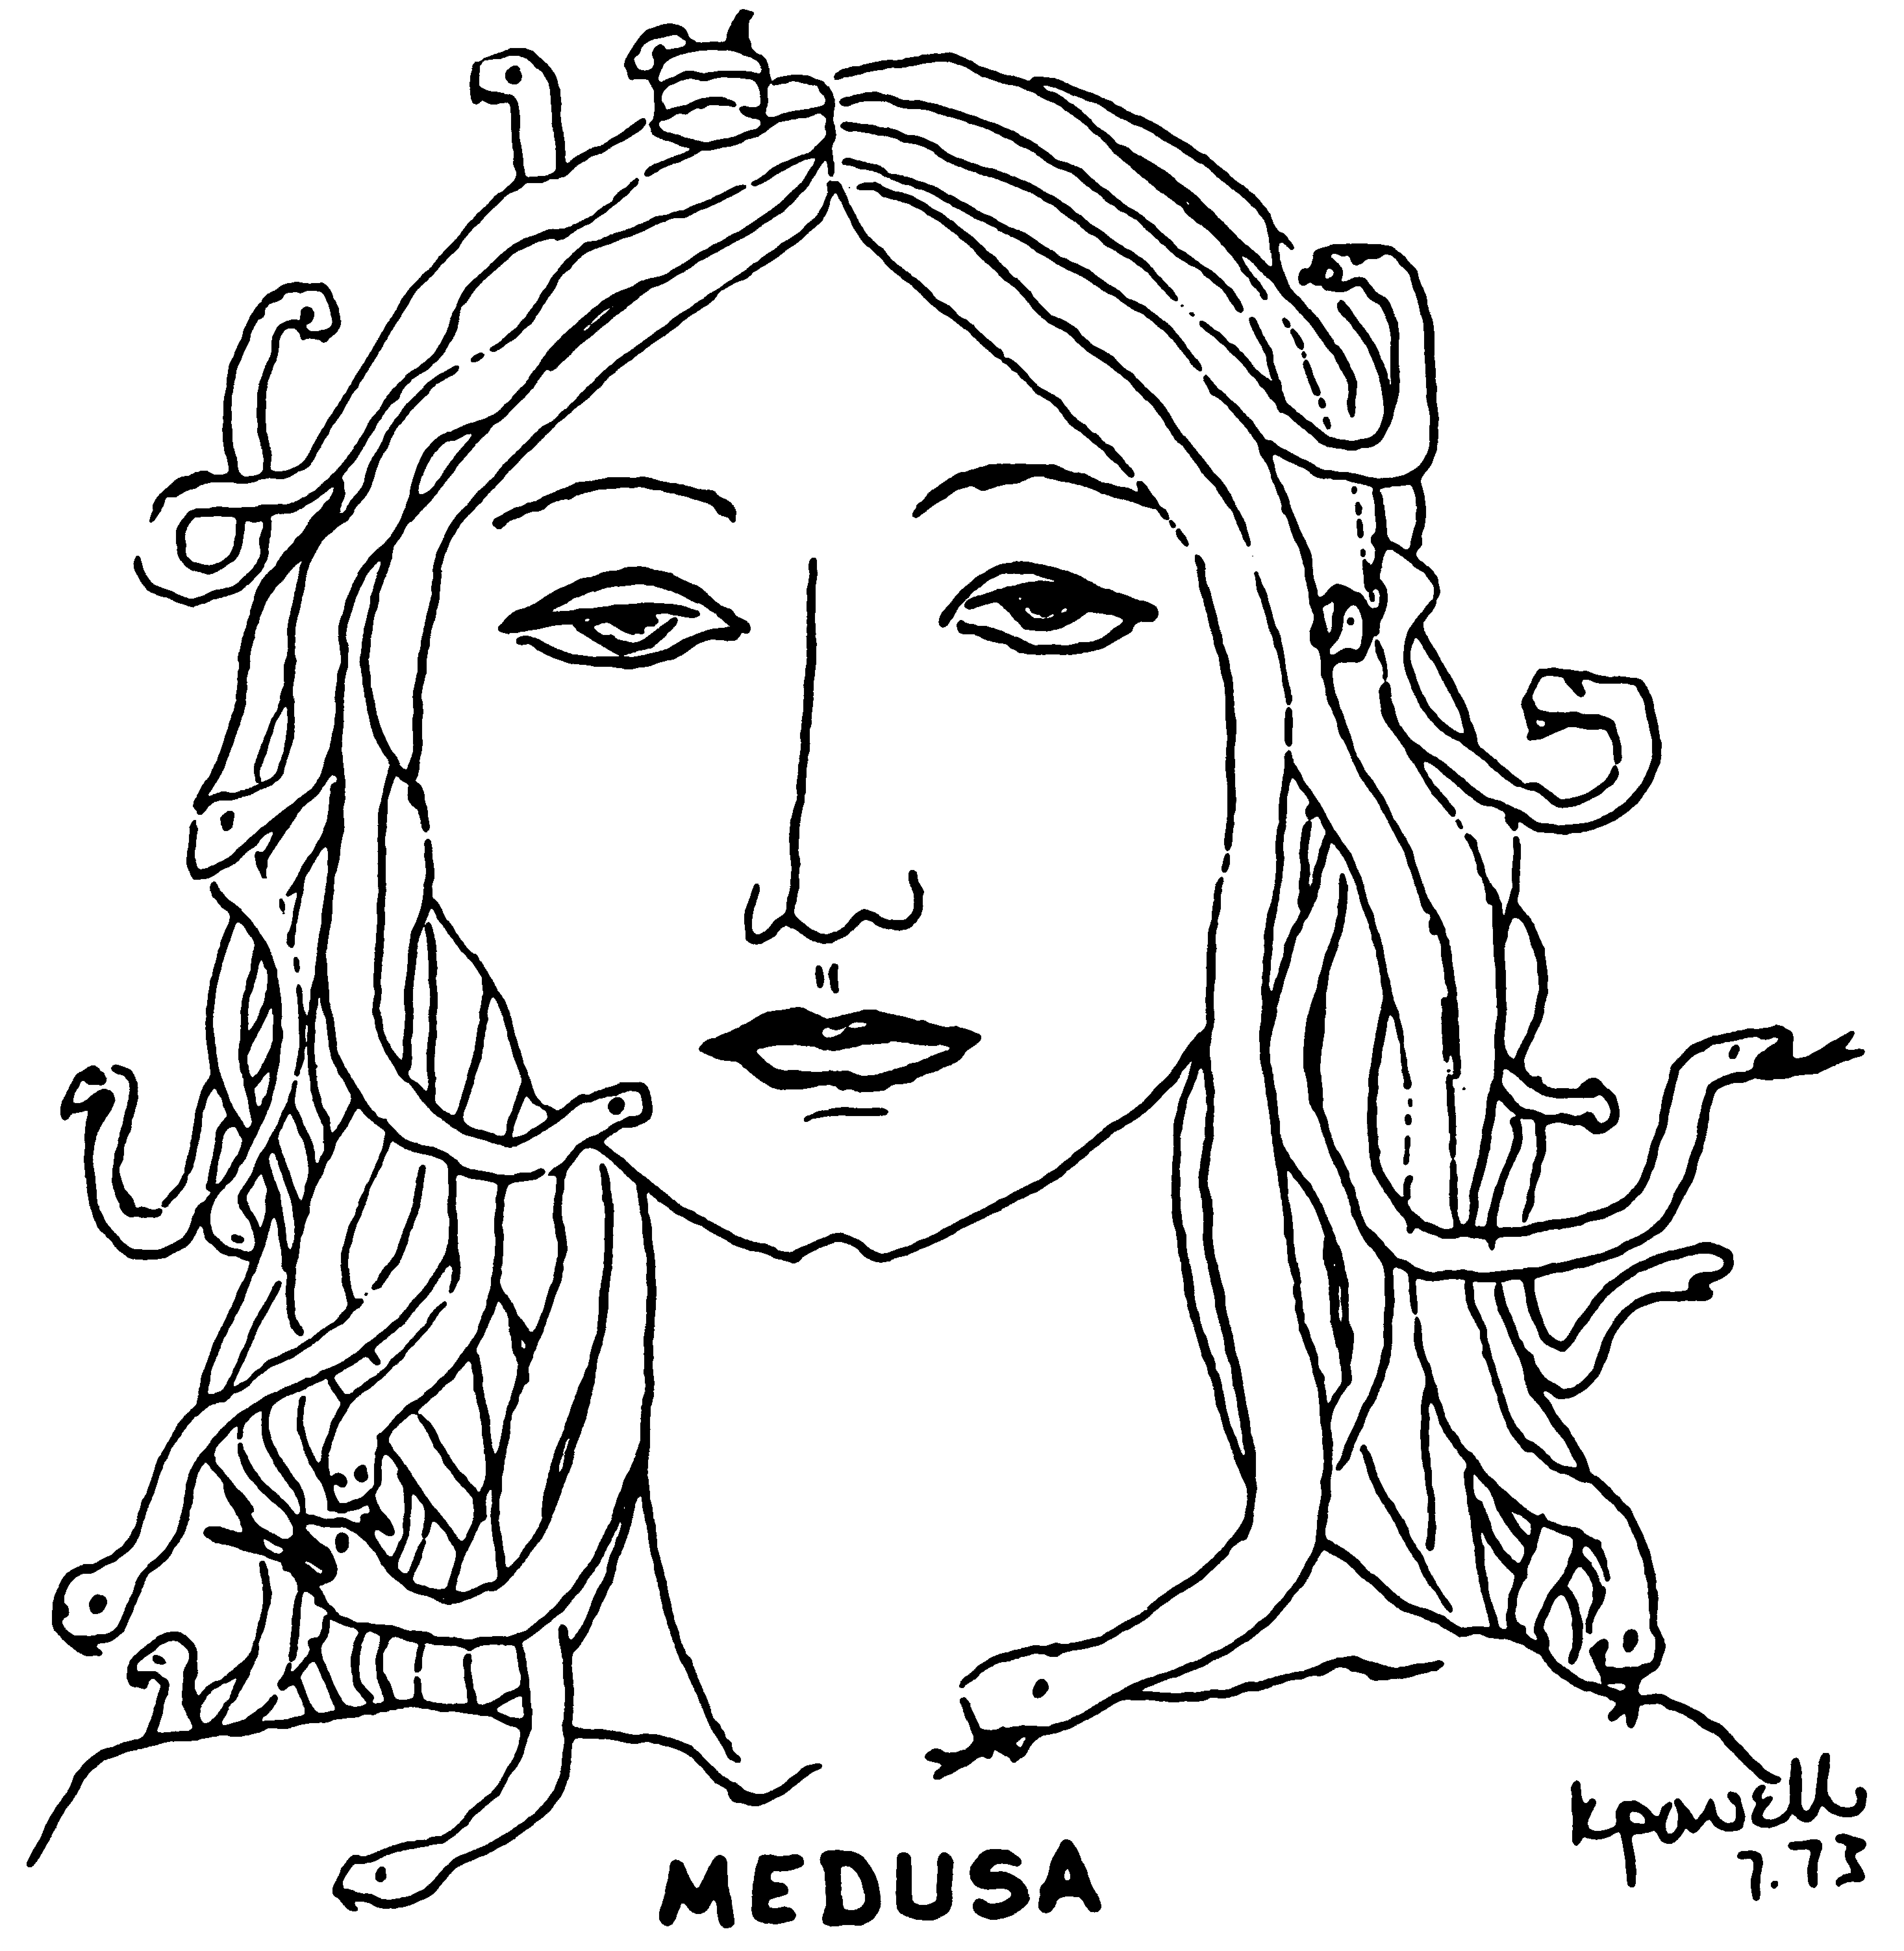
\includegraphics[scale=0.042]{./images/medusa.jpg}
\end{center}

\newpage

\begin{tabular}[t]{p{3cm}p{12cm}}
\multicolumn{2}{l}{\myunderline{\textbf{Table des Capacités Extraordinaires}}} \\
\textbf{\myunderline{Jet de dé}} & \myunderline{\textbf{Capacité}} \\
01--10 & Clairaudience \\
11--20 & Clairvoyance \\
21--30 & Perception extra-sensorielle (ESP) \\
31--40 & Télépathie \\
41--50 & Télékinésie \\
51--59 & Téléportation \\
60--68 & Vision rayons X \\
69--77 & Génération d'illusions \\
78--82 & Lévitation \\
83--87 & Vol \\
88--92 & Soins (1 point par 6 tours ou 6 points par jour) \\
93--97 & 1--4 fois la force normale pendant 1--10 tours, peut être employé une fois par jour \\
98-99 & Refaire deux jets en ignorant les jets au-dessus de 97 \\
\hspace{0.4cm}00 & Refaire trois jets en ignorant les jets au-dessus de 97 \\
\end{tabular}

\medskip

Tous les Pouvoirs Primaires et Capacités Extraordinaires sont transmis à l'utilisateur de l'épée. Si vous tirez la même capacité deux fois , cela signifie que la capacité est doublée en termes de force, de portée, de précision, et.

\bigskip

\myunderline{\textbf{Egoïsme}} : seules les épées avec une Intelligence de 7 ou plus ont un score d'Egoïsme. L'Egoïsme est compris dans l'intervalle 1--12, plus le nombre est grand et plus grand est l'Egoïsme de l'épée. L'Egoïsme de l'épée peut lui faire faire les choses suivantes :

\begin{enumerate}
\item Obliger l'utilisateur à se défaire de meilleures armes,
\item Mettre l'utilisateur dans des situations très dangereuses afin d'exalter son rôle dans le combat,
\item Se laisser capturer par un personnage ou une créature de niveau plus élevé qui est plus proche de l'esprit de l'épée,
\item Se laisser capturer par un personnage ou une créature de niveau plus faible dans le but d'exercer un plus grand contrôle sur son utilisateur, et
\item Exiger qu'une partie des trésors conquis lui soit consacré, sous la forme de meilleurs fourreaux, d'incrustations de joyaux, ou de dispositifs magiques pour la garder lorsque personne ne l'utilise.
\end{enumerate}

A chaque moment où une situation se présente durant laquelle une des possibilités listées ci-dessus existe, l'Egoïsme de l'épée intervient. Ce dernier influencera toujours sa relation à l'utilisateur, bien que de vrais rapports puissent voir le jour si l'alignement et les buts du personnage/utilisateur coïncident avec l'\myunderline{origine/objectife} de l'épée. La détermination de chaque facteur est décrite ci-après:

\begin{center}
\begin{minipage}{0.8\linewidth}
\textbf{Influence de l'Egoïsme dans des Situations Clef} : l'arbitre additionne l'Intelligence et l'Egoïsme de l'épée (entre 8 et 24) et ajoute 1 pour chaque Capacité Extraordinaire (entre 1 et 4 si applicable). Le total (dans l'intervalle 8--28) est comparé à la somme de l'Intelligence et de la Force du personnage (6--36) modifié par une variable basée sur l'état physique de l'utilisateur. Si le personnage est frais et relativement exempt de dommages (moins de 10\% de dommages), il faut \myunderline{ajouter} 1--6 points à son total (pour arriver à un intervalle de 7--42). S'il est mentalement ou physiquement fatigué, ou s'il a subi des dommages compris entre 10\% et 50\%, il faut \myunderline{déduire} 1--4 points de son total (pour arriver à un intervalle de 2--35). Si les dommages subis dépassent les 50\%, ou le personnage a été sous le coup d'une tension mentale sévère venant d'une forme de magie, il faut \myunderline{déduire} 2--8 points (pour arriver à un intervalle de 0--34).

\bigskip

{\parindent0.5cm \begin{tabular}{ll}
\textbf{\myunderline{Différence}} & \myunderline{\textbf{Résultat}} \\
6 ou plus & Le plus haut score l'emporte \\
2--5 & 75\% de chances que le plus haut score l'emporte \\
0--1 & 50\% de chances pour chacun \\
\end{tabular}}

\bigskip

\textbf{L'Egoïsme dans les relations au long cours avec l'utilisateur} : cette détermination est assez simple, car elle est basée sur la comparaison du score d'Egoïsme de l'épée (1--12) avec le niveau du combattant l'utilisant. Consultez la table des \myunderline{Situations Clef} ci-dessus. Si l'une des parties a une différence positive de 6 ou plus, celle-ci l'emportera toujours et plus aucun test (incluant les Situations Clef) ne sera nécessaire. Une différence positive de 2--5 indiquera que celle ayant le plus haut score l'emporte généralement, et les tests ne devront être effectués que dans les Situations Clef. Une différence de 0--1 indique un combat continu entre l'épée et son utilisateur, et durant les situations stressantes, les deux devraient être testés afin de déterminer qui l'emporte.

\end{minipage}
\end{center}

\myunderline{\textbf{Origine/Objectif}} : naturellement, l'origine de chaque épée est la Loi, la Neutralité ou le Chaos, mais certaines de ces armes sont forgés par des forces plus puissantes pour un objectif particulier. Pour déterminer si une épée possède un tel objectif, faire un jet de pourcentage et un jet de 91 ou plus indique que l'épée possède une mission spéciale. Les épées avec des objectifs spéciaux voient automatiquement leur score l'Intelligence et d'Egoïsme poussés au maximum et elles gagnent une capacité additionnelle :

\bigskip

{\parindent1cm \textbf{Loi}: capacité de paralyser les opposants chaotiques,

\textbf{Neutralité} : ajoute +1 à tous les jets de sauvegarde,

\textbf{Chaos} : capacité de désintégrer les opposants loyaux.}

\bigskip

La capacité spéciale ne sera applicable que pour ceux que l'épée a été chargée de détruire, ou ceux qui les servent.

\myunderline{\textbf{Objectifs}}:

\medskip

{\parindent1.5cm\begin{tabular}{p{4.6cm}p{4.6cm}p{4.6cm}}
Tuer les magiciens & Tuer les combattants & Vaincre la Loi \\
Tuer les clercs & Tuer les monstres & Vaincre le Chaos \\
\end{tabular}}

\bigskip

Ainsi, une épée au service de la Loi ayant pour but de tuer les magiciens (chaotiques) les paralysera ainsi que leurs sbires, mais elle n'utilisera pas ses pouvoirs de paralysie contre un géant errant. Néanmoins, les épées ayant un objectif large utiliseraient leurs pouvoirs pour vaincre tous les opposants de nature Loyale ou Chaotique. Les épées ayant un objectif spécial de Neutralité agiront contre la Loi et le Chaos de la même manière. Les épées ayant un objectif spécial chercheront toujours à l'accomplir, et chaque tentative des utilisateurs de le contrer se soldera immédiatement par un test d'influence.

\bigskip

\myunderline{\textbf{EPEES, BONUS AUX DOMMAGES}} : Les épées reçoivent toutes des bonus pour ce qui est de la probabilité de toucher un opposant, mais certaine sd'entre elles reçoivent aussi un bonus aux dommages quand elles touchent. Ces épées sont celles qui ont un +2 ou +3 contre certaines créatures, mais pas celles qui ont un bonus général de +2 ou +3.
}% parindent


%==========================================================================SECTION
\newpage
\section*{Glossaire anglais-français }

{\parindent0cm

\textbf{Animal Telepathy} : Télépathie animale. Pouvoir psionique.

\textbf{Astral projection} : Projection astrale. Pouvoir psionique.

\textbf{Aura Alteration} : Altération de l'aura. Pouvoir psionique.

\textbf{Body control} : Contrôle du corps. Pouvoir psionique.

\textbf{Body Equilibrium} : Changer le poids du corps. Pouvoir psionique.

\textbf{Body Weaponry} : Corps comme arme. Pouvoir psionique.

\textbf{Cell adjustment} : Contrôle cellulaire. Pouvoir psionique.

\textbf{Clairaudience} : Clairaudience. Pouvoir psionique.

\textbf{Clairvoyance} : Clairvoyance. Pouvoir psionique.

\textbf{Detection of Evil/Good} : Détection du Mal/du Bien. Pouvoir psionique.

\textbf{Detection of Magic} : Détection de la magie. Pouvoir psionique.

\textbf{Dimension Door} : Porte dimensionnelle. Pouvoir psionique.

\textbf{Dimension Walking} : Marche dimensionnelle. Pouvoir psionique.

\textbf{Domination} : Domination. Pouvoir psionique.

\textbf{Empathy} : Empathie. Pouvoir psionique.

\textbf{Energy control} : Contrôle de l'énergie. Pouvoir psionique.

\textbf{ESP} : Perception extrasensorielle. Pouvoir psionique.

\textbf{Etherealness} : Transformation éthérée. Pouvoir psionique.

\textbf{Expansion} : Expansion. Pouvoir psionique.

\textbf{Hypnosis} : Hypnose. Pouvoir psionique.

\textbf{Invisibility} : Invisibilité. Pouvoir psionique.

\textbf{Levitation} : Lévitation. Pouvoir psionique.

\textbf{Mass Domination} : Domination des masses. Pouvoir psionique.

\textbf{Mind Bar} : Barrière mentale. Pouvoir psionique.

\textbf{Mind Over Body} : Contrôle de l'esprit sur le corps. Pouvoir psionique.

\textbf{Molecular Agitation} : Agitation moléculaire. Pouvoir psionique.

\textbf{Molecular Manipulation} : Manipulation moléculaire. Pouvoir psionique.

\textbf{Molecular Rearrangement} : Réarrangement moléculaire. Pouvoir psionique.

\textbf{Precognition} : Prémonition. Pouvoir psionique.

\textbf{Probability Travel} : Voyage probabiliste. Pouvoir psionique.

\textbf{Reduction} : Réduction. Pouvoir psionique.

\textbf{Roc} : Rokh, oiseau fabuleux des contes d'origine persane et indienne écrit en langue arabe.

\textbf{Shape Alteration} : Altération de la forme. Pouvoir psionique.

\textbf{Suspend Animation} : Hibernation. Pouvoir psionique.

\textbf{Telekinesis} : Télékinésie. Pouvoir psionique.

\textbf{Telepathic Projection} : Projection télépathique. Pouvoir psionique.

\textbf{Teleportation} : Téléportation. Pouvoir psionique.

}% parindent













\begin{verbatim}
---
tags:
    - Ambre
    - D&D
    - Zelazni
---

# Vocabulaire

Alors que l'on dit plutôt en français, "pouvoirs psychiques", le terme américain "psionic" est entré progressivement dans le vocabulaire des jeux de rôles, souvent en étant francisé en "psionique". Dans cet article, nous nous limiterons à l'usage du terme "psychique" en français, le terme "psionic" étant réservé à la citation d'ouvrages en anglais.

# 1976 - OD&D au début de tout (comme souvent)

## Introduction

![Alt text](../images/eldritch-wizardry.png)

En 1976 sort le livre VI de *Dungeons & Dragons* avec le titre *Eldritch Wizardry* cosigné de [Gary Gygax](https://github.com/orey/DandD/tree/master/GaryGygax) et de Brain Blume. Ce livre d'une soixantaine de pages contient essentiellement des suppléments sur les pouvoirs psychiques, sur le druide en tant que classe de personnage et sur les démons.

Ledit supplément est disponible sur [archive.org](https://archive.org/details/tsr02005supplement3eldritchwizardy). Il n'a pas été traduit en français à ma connaissance alors que les règles de OD&D l'ont été : voir sur le très bon site [La Forge de papier](http://la-forge-de-papier.over-blog.com/2017/09/donjons-dragons-la-boite-blanche-elle-aussi-en-francais.html).

Il semble que ce soit la première apparition des pouvoirs psychiques dans le monde du JDR. Leur apparition au sein de *D&D* a quelque chose d'étrange, car on pourrait y voir une collision de diverses influences dans la fantasy: le médiéval-fantastique qui favorise la magie et les pouvoirs psychiques qui sent plus le JDR contemporain ou futuriste.

D&D propose les pouvoirs psy comme un genre de supplément optionnel pour "pimenter" les parties. L'introduction de 1976 de [Tim Kask](https://en.wikipedia.org/wiki/Tim_Kask) dudit livre est amusante :

*L'introduction du combat psionique s'attache à redynamiser des jeux devenus ternes. Cela ouvre des possibilités inédites à la fois pour les joueurs et le MD et, ce faisant, cela permet de se reconnecter à l'un des thèmes favoris des écrivains de science-fiction et de fantasy : les pouvoirs inconnus de l'esprit.*

Pour autant, en lisant entre les lignes, l'introduction des démons dans le jeu semble pousser Gygax à créer les règles des pouvoirs psychiques, mieux adaptés, selon lui, à représenter les pouvoirs de certains démons.

Comme souvent dans OD&D, les règles sont confuses, incomplètes, éclatées dans le tout le livret, entrecoupées de choses qui n'ont rien à voir (le Druide, un système de combat alternatif basé sur la **Dextérité Ajustée**, etc.). Au niveau édition, *Eldritch Wizardry* est un des pires exemples de l'époque.

## Obtention des Pouvoirs Psychiques (PoP)

A la création du PJ, un score de 15 ou plus dans INTelligence, WISdom ou CHArisma donne la possibilité de tester si le personnage dispose d'un pouvoir psy (si le personnage est humain). Il est nécessaire de faire 91 ou plus sur 1d100 pour que ce soit le cas. Les moines et les druides ne peuvent pas avoir de pouvoirs psychiques.

Si le personnage est éligible, il faut faire un nouveau jet de 1d100 pour déterminer le **potentiel psychique** (PP, purement aléatoire). Suivant le PP, le PJ obtient un malus ou un bonus pour avoir des **pouvoirs psychiques** (PoP, de -6% à +3%).

| PP (1d100) | Bonus/Malus au jet d'obtention de PoP (BMPoP) |
|------------|-----------------------------------------------|
| 01–10      | -6% par niveau (cumulatif)                    |
| 11–25      | -5% par niveau (cumulatif)                    |
| 26–50      | -4% par niveau (cumulatif)                    |
| 51–75      | Aucun                                         |
| 76–90      | +1% par niveau (cumulatif)                    |
| 91–99      | +2% par niveau (cumulatif)                    |
| 00         | +3% par niveau (cumulatif)                    |

La chance de base pour avoir un PoP est de 10% + BMPoP par niveau. Ainsi, un perso du 4ème niveau avec un PP de 90 aura une base de 10 + 1 = 11 soit 11 x 4 = 44% de chances d'avoir un PoP. Cela veut dire aussi qu'un personnage de niveau 10 aura 100% d'avoir un PoP.

Notons enfin que donc, ce jet se produit à chaque changement de niveau.

Cerise sur le gâteau : si le PJ obtient un PoP, alors s'il réussit un jet de 1d100 sous son PP, il en a automatiquement un second !

Nous sommes en plein dans le monde Gygaxien des **règles gigognes** :

* R1 : INT ou WIS ou CHA > 15,
* R2 : Si R1 OK, jet de 1d100 pour PP et BMPoP,
* R3 : Quand R2 OK, jet de BMPoP pour obtenir un PoP,
* R4 : Si R3 OK, si succès, alors jet de PP pour obtenir un second PoP.

Nous verrons apparaître ce genre de règles gigognes dans les autres éditions de D&D signées de Gygax.

## Pouvoirs psychiques (PoP)

### Liste des pouvoirs

La liste originale est présentée ci-dessous.

![Listedescompetencespsioniques](../images/od&d-psionics.png)

La liste des PoP est fournie ci-dessous, retriée par type (interprétation personnelle) et par classe de personnages.

| Pouvoir Psychique (PoP)           | Type | Guerriers & Voleurs | Magiciens  | Clercs     |
|-----------------------------------|------|---------------------|------------|------------|
| Réduction                         | A    | 1 Oui (B)           | 1 Oui (B)  |            |
| Expansion                         | A    | 2 Oui (B)           | 2 Oui (B)  |            |
| Lévitation                        | A    | 3 Oui (B)           | 3 Oui (B)  | 1 Oui (B)  |
| Changer le poids du corps         | A    | 4 Oui (B)           |            | 2 Oui (B)  |
| Corps comme arme                  | A    | 5 Oui (B)           |            |            |
| Réarrangement moléculaire         | A    | 6 Oui (S)           |            | 3 Oui (S)  |
| Manipulation moléculaire          | A    | 7 Oui (S)           |            |            |
| Contrôle du corps                 | A    | 8 Oui (S)           |            |            |
| Barrière mentale                  | A    | 9 Oui (S)           |            |            |
| Agitation moléculaire             | A    |                     | 4 Oui (B)  |            |
| Altération de la forme            | A    |                     | 5 Oui (S)  |            |
| Contrôle cellulaire               | A    |                     |            | 4 Oui (B)  |
| Contrôle de l'esprit sur le corps | A    | 10 Oui (B)          |            | 5 Oui (B)  |
| Invisibilité                      | A    | 11 Oui (B)          |            |            |
| Hibernation                       | A    | 12 Oui (B)          |            |            |
| Télékinésie                       | A    | 13 Oui (S)          | 6 Oui (S)  |            |
| Contrôle de l'énergie             | A    | 14 Oui (S)          |            |            |
| Domination                        | B    | 15 Oui (B)          |            | 6 Oui (B)  |
| Hypnose                           | B    |                     | 7 Oui (B)  | 7 Oui (B)  |
| Projection télépathique           | B    |                     | 8 Oui (S)  | 8 Oui (S)  |
| Altération de l'aura              | B    |                     |            | 9 Oui (S)  |
| Domination des masses             | B    |                     |            | 10 Oui (S) |
| ESP                               | B    |                     | 9 Oui (B)  | 11 Oui (B) |
| Empathie                          | B    |                     |            | 12 Oui (S) |
| Télépathie animale                | B    |                     |            | 13 Oui (B) |
| Prémonition                       | C    | 16 Oui (B)          | 10 Oui (S) | 14 Oui (S) |
| Clairaudience                     | C    | 17 Oui (B)          | 11 Oui (B) |            |
| Clairvoyance                      | C    | 18 Oui (B)          | 12 Oui (B) |            |
| Détection du mal/du bien          | C    |                     | 13 Oui (B) | 15 Oui (B) |
| Détection de la magie             | C    |                     | 14 Oui (B) |            |
| Marche dimensionnelle             | D    | 19 Oui (S)          |            | 16 Oui (S) |
| Projection astrale                | D    | 20 Oui (S)          | 15 Oui (S) | 17 Oui (S) |
| Porte dimensionnelle              | D    |                     | 16 Oui (S) |            |
| Téléportation                     | D    |                     | 17 Oui (S) |            |
| Substance éthérée                 | D    |                     | 18 Oui (S) |            |
| Voyage probabiliste               | D    |                     |            | 18 Oui (S) |

Nous pouvons classer ces pouvoirs en plusieurs catégories (ce n'est pas dans le livre original) :

* A : Contrôle de la matière au niveau moléculaire, voire atomique,
* B : Contrôle via l'esprit de l'esprit,
* C : Sens,
* D : Voyage psychique.

Les pouvoirs sont présents chez les types de personnages soient au niveau Basique (B) soit au niveau Supérieur (S). Le fait qu'un PoP soit Supérieur ne se traduit (dans les règles) que par le fait qu'elle soit détectable par un autre personnage ayant des pouvoirs psy au double de la portée du pouvoir (voir plus bas détection des pouvoirs psychiques).

Les PJ ne peuvent pas avoir plus de PoP Supérieurs que de PoP Basiques.

Cette distinction est peu développée et on imagine que le but était d'avoir la possibilité de deux puissances différentes dans les mêmes pouvoirs. Par contre, les pouvoirs eux-mêmes n'utilisent pas cette distinction.

La détermination des PoPs est aléatoire mais il est suggéré de restreindre le choix à des types de PoP cohérents.

### A - Contrôle de la matière et de l'énergie

On retrouve dans cette dimension pas mal de pouvoirs :

* Réduction ;
* Expansion ;
* Lévitation, qui est un moyen de changer le poids du corps ;
* Changer le poids du corps (*Body Equilibrium*), notamment pour marcher sur l'eau ;
* Corps comme arme (*Body Weaponry*) ;
* Réarrangement moléculaire, qui transforme les métaux ;
* Manipulation moléculaire, qui permet de rendre fragile différentes matières dures ;
* Contrôle du corps, qui permet d'adapter le corps à des conditions extrêmes comme le froid extrême, le feu, les fumées empoisonnées, etc. ;
* Barrière mentale ;
* Agitation moléculaire, agit un peu comme un four à micro-ondes ;
* Altération de la forme, pour se changer en quelqu'un d'autre ;
* Contrôle de l'esprit sur le corps, pour se passer de manger, de boire et de dormir ;
* Invisibilité ;
* Hibernation (*Suspend Animation*), ou comment suspendre ses fonctions vitales ;
* Télékinésie, contrôle du mouvement des objets par la pensée ;
* Contrôle de l'énergie, ou comment dissiper des énergies agressives ;
* Contrôle cellulaire (*Cellular Adjustment*), qui permet de soigner les blessures et les maladies.

### B - Contrôle via l'esprit de l'esprit

On retrouve les pouvoirs suivants :

* Domination, pour forcer une personne à faire ce que le PJ souhaite ;
* Hypnose, contrôle des esprits faibles ;
* Projection télépathique, envoyer des messages ou influence une personne ;
* Altération de l'aura ;
* Domination des masses ;
* ESP ;
* Empathie ;
* Télépathie animale.

### C - Sens

On retrouve les pouvoirs suivants :

* Prémonition ;
* Clairaudience ;
* Clairvoyance ;
* Détection du mal/du bien ;
* Détection de la magie.

### D - Voyage psychique

* Marche dimensionnelle ;
* Projection astrale ;
* Porte dimensionnelle
* Téléportation
* Substance éthérée ;
* Voyage probabiliste, une projection astrale avec le corps permettant de passer à travers les plans et les mondes parallèles (comme dans la *Saga des Princes d'Ambres* de Zelazni).

## Modes d'Attaque et Modes de Défense

Une fois que le PJ a son premier PoP, il gagne son premier **Mode d'Attaque** psychique (MA) : *Explosion psionique* (voir tableau ci-dessous).

Les autres MA sont gagnés tous les 4 PoP (5 pour les Guerriers).

Cette dernière consigne est un peu vague. Elle sous-entend que, lors du passage de niveau, le PJ ayant des pouvoirs psychiques va refaire un test pour avoir un nouveau PoP (sachant qu'il peut en obtenir au maximum deux par niveau). Il gagnera un mode d'attaque alors en fonction du nombre de PoP dont il dispose.

Concernant les **Modes de Défense** (MD), encore une fois les règles ne sont pas claires. Il est dit qu'ils sont acquis à raison de un tous les 3 PoP acquis (4 pour les Guerriers).

Comme les PJs ayant des pouvoirs psychiques sont capables de combattre psychiquement, il faut supposer que les MDs marchent comme pour les MAs et que le PJ gagne son premier MD avec son premier PoP, puis ensuite tous les 3 (ou 4) PoP acquis.

Une autre interprétation possible serait qu'il faut vraiment avoir 3 ou 4 PoP pour gagner son premier MD. Je trouve cette interprétation un peu bizarre au regard de la suite qui présuppose, dans le combat psionique, que l'attaquant psy a un MA et que le défenseur a un MD. Un défenseur ayant des pouvoirs psychiques sans MD ouvre une brèche dans le système.

Il n'est pas expliqué comment les MA/MD sont attribués : aléatoirement (D6 en rejouant le 6) ou séquentiellement, en utilisant les lettres, ou par simple choix. Comme la puissance de ces attaques est diverse et non linéaire, je pense pas que les lettres soient très importantes pour les MA. Pour les MD, il y a une certaine progression. Au DM de choisir son mode d'attribution.

La liste des modes d'attaque et de défense est présentée ci-dessous avec leur coût en **Force Psionique** entre parenthèses.

| Modes d'Attaque (MA), toutes classes     | Modes de Défense (MD), toutes classes |
|------------------------------------------|---------------------------------------|
| A. Explosion psionique (20)[x3]          | F. Esprit vide (1)                    |
| B. Poussée de l'esprit (10)[x1]          | G. Bouclier de pensée (2)             |
| C. Coup de fouet sur l'ego (15)[x3]      | H. Barrières mentales (4)             |
| D. Imposition d'identité (10)[x1]        | I. Forteresse intellectuelle (7)      |
| E. Ecrasement psychique (25&spades;)[x3] | J. Tour de volonté de fer (10)        |

&spades; Si le PJ possède moins de 25 points de FP, il est demandé au MJ de "modifier la probabilité de succès de manière *ad hoc*".

L'utilisation des MAs peut être détectée par un PJ ou PNJ ayant des pouvoirs psychiques. Le facteur entre crochets donne le multiplicateur de portée du MA dans lequel le PJ ou PNJ peut détecter son usage. Pour mémoire, les pouvoirs

## Force Psionique (FP), Force Psionique d'Attaque (FPA) et de Défense (FPD)

Les formules sont les suivantes :

* FPA = PP + 2 x nombre(PoP) + 5 x nombre(MA) + 5 x nombre(MD)
* FPD = FPA
* FP = FPA + FPD = 2 x FPA

Ces scores serviront de réservoirs de points pour les attaques et les défenses psychiques en combat psychique, mais aussi pour les divers PoP que les PJs auront accumulés et dont le coût est expliqué dans les descriptions.

A chaque fois que de la FP est consommée, il faut répartir la consommation à 50%-50% entre la FPA et la FPD, cela pour toutes les consommations. En gros, la FP est un réservoir de points divisés en deux avec une consommation égale dans les deux sous-réservoirs (cela vaut aussi pour la consommation des points en combat, soit avec les MA et MD).

La FP se récupère assez vite en cessant toute activité psychique et en suivant les indications de la table suivante.

| Activité                            | Gain en FP          |
|-------------------------------------|---------------------|
| Marcher, parler et autres activités | 6 points par heure  |
| Se reposer tranquillement           | 12 points par heure |
| Dormir                              | 24 points par heure |

## Détection des PoP et des MA

La table ci-dessous présente les règles de détection des PoP et MA (nous avons utilisé les lettres pour désigner les MA) de PJs ou PNJs ayant des pouvoirs psychiques et détectant dans leur voisinage des créatures utilisant des pouvoirs.

| Type                     | Niveau/Nom | Portée de la détection | % de base | Cumulatif par tour |
|--------------------------|------------|------------------------|-----------|--------------------|
| PoP                      | Basique    | Portée du pouvoir      | 10%       | Oui (+10%)         |
| PoP                      | Supérieur  | 2 x Portée du pouvoir  | 10%       | Oui (+10%)         |
| MA                       | A, C, E    | 3 x Portée du pouvoir  | 10%       | Oui (+10%)         |
| MA                       | B, D       | Portée du pouvoir      | 10%       | Oui (+10%)         |
| Objet psy                | -          | Portée du pouvoir      | 10%       | Oui (+10%)         |
| Sort (idem psy)          | -          | Portée du sort         | 10%       | Oui (+10%)         |
| Objet magique (idem psy) | -          | Portée du sort         | 10%       | Oui (+10%)         |

Si le pouvoir est utilisé en continu, alors les chances de détection dans le cadre de la portée de détection grandissent de 10% par tour.

La créature qui détecte ne pourra pas détecter un pouvoir qu'elle n'a pas, mais pourra, au premier tour détecter dans quelle direction le pouvoir est utilisé, et au second tour avec quelle puissance "relative" ce pouvoir est utilisé.

Les sorts qui sont similaires aux pouvoirs psychiques seront détectés de la même façon que lesdits pouvoirs. Les objets magiques qui ont les mêmes fonctions que les objets psychiques seront, eux-aussi, détectés de la même façon.

## Le PJ psionique selon OD&D

Le PJ psionique a donc les caractéristiques suivantes :

* PP avec BMPoP,
* Liste des PoPs,
* FP = FPA + FPD,
* Listes des MAs et MDs.

## Combat psychique




*En cours*

## Liens



<div class="mydate">03-20 juin 2023</div>


\end{verbatim}




\end{document}
